%For printing? \documentclass[a4paper,10pt,twoside]{article}
\documentclass[a4paper,10pt]{article}

\usepackage{ucs}
\usepackage{caption}
\usepackage{tipx}

\usepackage{xcolor}
\usepackage{fontenc}
\usepackage{graphicx}
\usepackage{subfigure}
\usepackage[subfigure]{tocloft}

\usepackage[dvips]{hyperref}
\usepackage[dcucite]{harvard}

\usepackage{wrapfig}

\usepackage{tikz}
\usetikzlibrary{calc,mindmap,backgrounds,arrows,shapes.multipart,fit,trees,%
positioning,arrows,chains,shapes.geometric,decorations.pathreplacing,%
decorations.pathmorphing,shapes,matrix,shapes.symbols}
\usepackage{pgf-umlcd}
\usepackage{scalefnt}

\usepackage{color}
\usepackage{alltt}
% Style definition file generated by highlight 3.0 beta, http://www.andre-simon.de/ 

% Highlighting theme definition: 

\newcommand{\hlstd}[1]{\textcolor[rgb]{0.23,0.22,0.21}{#1}}
\newcommand{\hlnum}[1]{\textcolor[rgb]{1,0,1}{#1}}
\newcommand{\hlesc}[1]{\textcolor[rgb]{1,0,1}{#1}}
\newcommand{\hlstr}[1]{\textcolor[rgb]{1,0,1}{#1}}
\newcommand{\hlpps}[1]{\textcolor[rgb]{1,0,1}{#1}}
\newcommand{\hlslc}[1]{\textcolor[rgb]{0,0.24,1}{#1}}
\newcommand{\hlcom}[1]{\textcolor[rgb]{0,0.24,1}{#1}}
\newcommand{\hlppc}[1]{\textcolor[rgb]{0.63,0.13,0.94}{#1}}
\newcommand{\hlopt}[1]{\textcolor[rgb]{0.23,0.22,0.21}{#1}}
\newcommand{\hllin}[1]{\textcolor[rgb]{0.24,0.23,0.22}{#1}}
\newcommand{\hlkwa}[1]{\textcolor[rgb]{0.65,0.16,0.21}{#1}}
\newcommand{\hlkwb}[1]{\textcolor[rgb]{0.18,0.55,0.34}{#1}}
\newcommand{\hlkwc}[1]{\textcolor[rgb]{0.34,0.18,0.55}{#1}}
\newcommand{\hlkwd}[1]{\textcolor[rgb]{0.23,0.22,0.21}{\bf{#1}}}
\definecolor{bgcolor}{rgb}{1,1,1}

% Symbol definitions
\newsavebox{\hlboxopenbrace}
\newsavebox{\hlboxclosebrace}
\newsavebox{\hlboxlessthan}
\newsavebox{\hlboxgreaterthan}
\newsavebox{\hlboxdollar}
\newsavebox{\hlboxunderscore}
\newsavebox{\hlboxand}
\newsavebox{\hlboxhash}
\newsavebox{\hlboxat}
\newsavebox{\hlboxbackslash}
\newsavebox{\hlboxpercent}
\newsavebox{\hlboxhat}
\setbox\hlboxopenbrace=\hbox{\verb.{.}
\setbox\hlboxclosebrace=\hbox{\verb.}.}
\setbox\hlboxlessthan=\hbox{\verb.<.}
\setbox\hlboxgreaterthan=\hbox{\verb.>.}
\setbox\hlboxdollar=\hbox{\verb.$.}
\setbox\hlboxunderscore=\hbox{\verb._.}
\setbox\hlboxand=\hbox{\verb.&.}
\setbox\hlboxhash=\hbox{\verb.#.}
\setbox\hlboxat=\hbox{\verb.@.}
\setbox\hlboxbackslash=\hbox{\verb.\.}
\setbox\hlboxpercent=\hbox{\verb.\%.}
\setbox\hlboxhat=\hbox{\verb.^.}
\def\urltilda{\kern -.15em\lower .7ex\hbox{\~{}}\kern .04em}


\renewcommand{\topfraction}{0.85}
\renewcommand{\textfraction}{0.1}
\renewcommand{\floatpagefraction}{0.75}

\title{Real-Time Interactive 3D Modelling with Commodity Hardware
\vspace{30pt}}
\author{Peter Coetzee\\Supervisor: Andrew Davison
\vspace{30pt}}
\date{June 2010}

\begin{document}
\pagenumbering{roman}
\maketitle

\vspace{50pt}

\begin{abstract}
A long-standing problem in Computer Vision has been recovery of scene geometry; in both controlled and (in many cases) arbitrary environments. With applications ranging from robot navigation to augmented reality in film and television, the process of taking a real-world object and representing it in 3D has enormous inherent value. Nevertheless, existing techniques all leave something to be desired; be it their cost, the limited range of their applicability, or their accuracy.

The theoretical approach outlined in this document aims to alleviate many of the aforementioned pitfalls of traditional methods, by utilising cheap commodity hardware for recognition, by creating a system that is robust in completely un-controlled environmental conditions, and by making use of both \textit{human} and \textit{machine} intelligence in the manners best suited to them.
\end{abstract}

\pagebreak
\tableofcontents
\pagebreak

\begingroup
\renewcommand*{\addvspace}[1]{}
\setlength{\cftbeforefigskip}{5px}
\listoffigures

\newpage
\pagenumbering{arabic}

\section{Motivation}
There are a deceptively large number of industries with an interest in producing accurate 3D models of objects in the real world. Engineers, for example, working on a CAD model of a product upgrade may want to scan the old product as a base template. The visual effects industry invests thousands of pounds in laser scans for every show they work on; it is critically important that ``digital doubles" (digital replications of human beings) are identical to the people they are based on, both for immersion and often for technical reasons too. It is not unusual for a VFX studio to take a live action scene and replace the actor with their digital double, so that (for example) shadows are cast correctly, or some particularly gruesome mutilation can occur (such as for Harvey Dent's character in the recent Dark Knight movie, seen in Figure~\ref{twoface}).

\begin{figure}[h]
  \begin{center}
    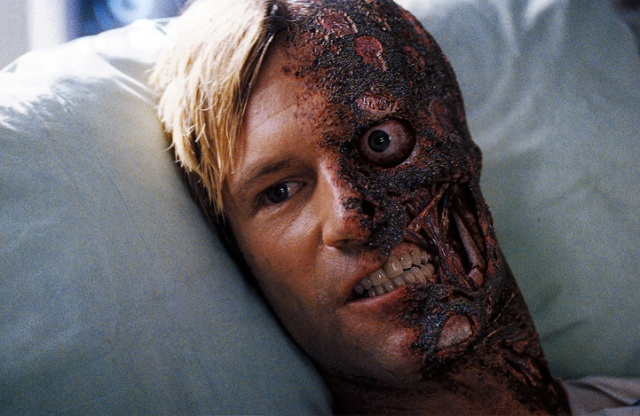
\includegraphics[width=340px]{twoface}
  \end{center}
  \vspace{-10pt}
  \caption{CGI Compositing: Digital Makeup for Harvey `Two-Face' Dent in The Dark Knight, \protect \copyright 2007 Warner Bros. Pictures}
  \label{twoface}
\end{figure}

Unless a studio owns the (typically expensive) equipment themselves, it can take weeks to get results back from 3rd party LIDAR scanning - if they had a means by which to create accurate models quickly and cheaply, they could do away with this expense altogether. In conversations with VFX professionals it emerges that the real challenge is to get an accurate \textit{proportional} reconstruction; artistic modelling can fill in as much detail as is desired, but to get the model in proportion a physical scan is required, by way of a foundation.

Furthermore, an increasing number of desktop applications are being produced to allow users to add models to their favourite games and social experiences; from Second Life to Quake, more people are learning 3D modelling and texture artistry. If they had a way of getting real-life objects into their games without having to undergo the horrifically steep learning curve of tools like Autodesk Maya or Mudbox, they would jump on the opportunity.

\clearpage

\section{Background}

As mentioned above, there are a variety of approaches to this well-studied problem available today. These solutions are typically selected to fit the particular use-case for the 3D model; their various strengths and weaknesses tend to recommend one over the other in any given situation.


\subsection{LIDAR}

\begin{wrapfigure}{r}{80pt}
  \vspace{-30pt}
  \begin{center}
    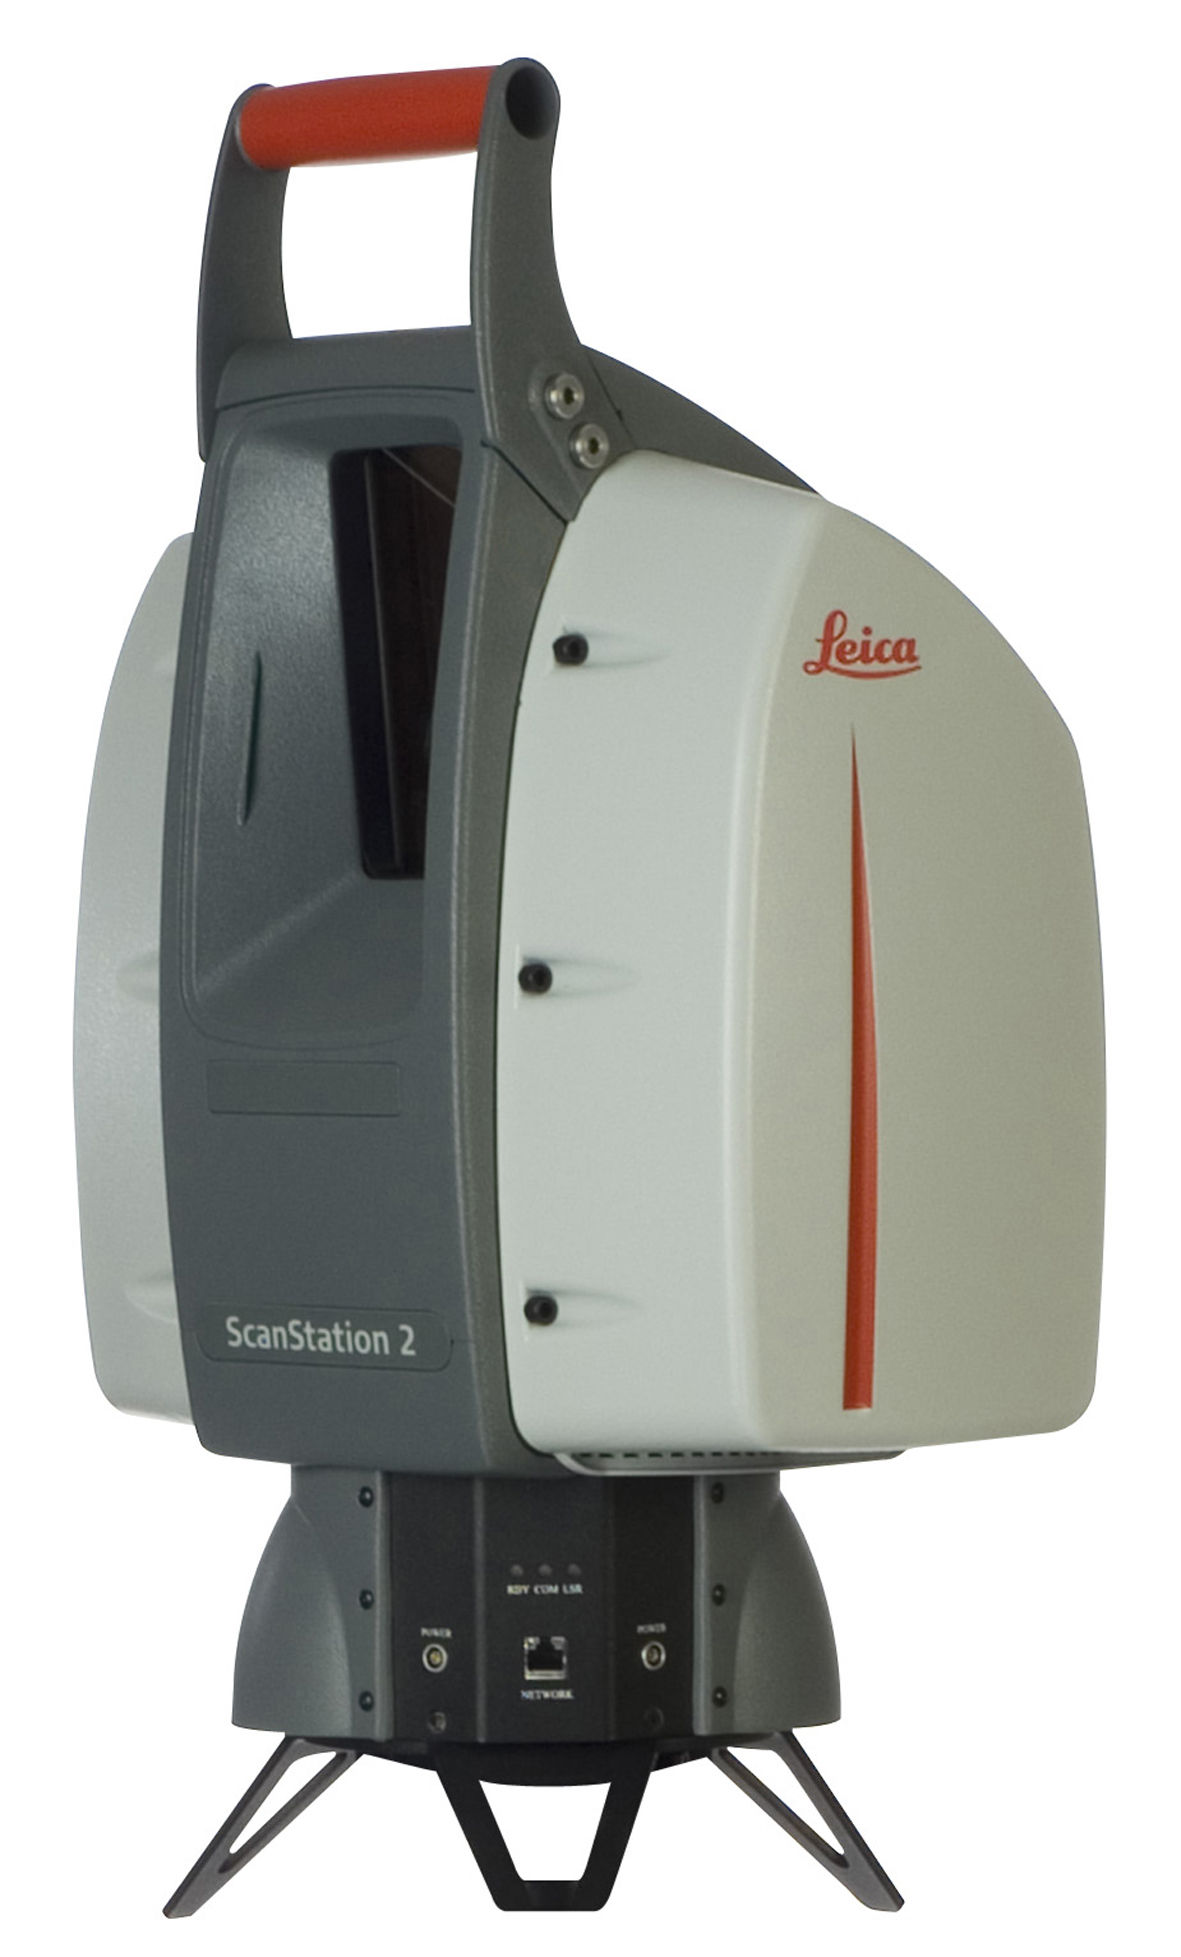
\includegraphics[width=80pt]{scanstation}
  \end{center}
  \caption{A Leica LIDAR Scanner}
  \label{scanstation}
  \vspace{-10pt}
\end{wrapfigure}

One common system used in the visual effects industry is LIDAR capture \cite**{lidar}, in which a scanning laser is used to trace the distance between it and the target object.
The object (or the scanner) is typically rotated during this process in order to generate a dense, 360$^\circ$ point-cloud representation of the scanned object. This technique, while expensive, is applicable in a variety of scenarios; from high-resolution facial capture through to large scale airborne ground topology scanning. This process requires little user intervention, and generates a large amount of data relatively quickly. However, much post-processing of this data is typically required; as it is a slightly noisy point-cloud, it must be cleaned up before it can be used in any real application. Furthermore, this cloud of points is not, by itself, geometry; it is more a set of candidate vertices for geometry, many of which will be discarded as they lie on surfaces. As a result, steps must be taken to generate surfaces in 3D which will fit these points.

\subsection{Automated Vision-Based Reconstruction}

One set of potentially valuable solutions which have received a lot of research attention recently are those around computer vision based systems. These show promise, in that they are based on much simpler hardware than LIDAR systems, instead focussing their complexity in intelligent software to analyse full colour imagery and extract the geometry from it. They are often based on using either a stereo camera, and thus using the fixed separation of the lenses to recover depth data, or augmenting a single lens with a laser rangefinder (a sort of vision-augmented LIDAR system). The details of implementation of such systems varies wildly. On one end of the scale, Photosynth \cite**{photosynth} employs heavy vision processing on still photographs of a given scene (potentially taken with different cameras, lenses, and in varying lighting conditions) and constructs a 3D montage of these images in order to give the effect of a textured 3D model. As part of this process, it actually constructs a coloured point cloud (as seen in Figure~\ref{photosynthcloud}), in much the same fashion as a LIDAR scan, and matches these points probabilistically to features in the set of input images. Work has been done \cite**{multistereo} on a similar approach with the goal of constructing arbitrary 3D surfaces, rather than just interpolation of the views presented by a finite set of images.

\begin{figure}
  \vspace{-35pt}
  \begin{center}
    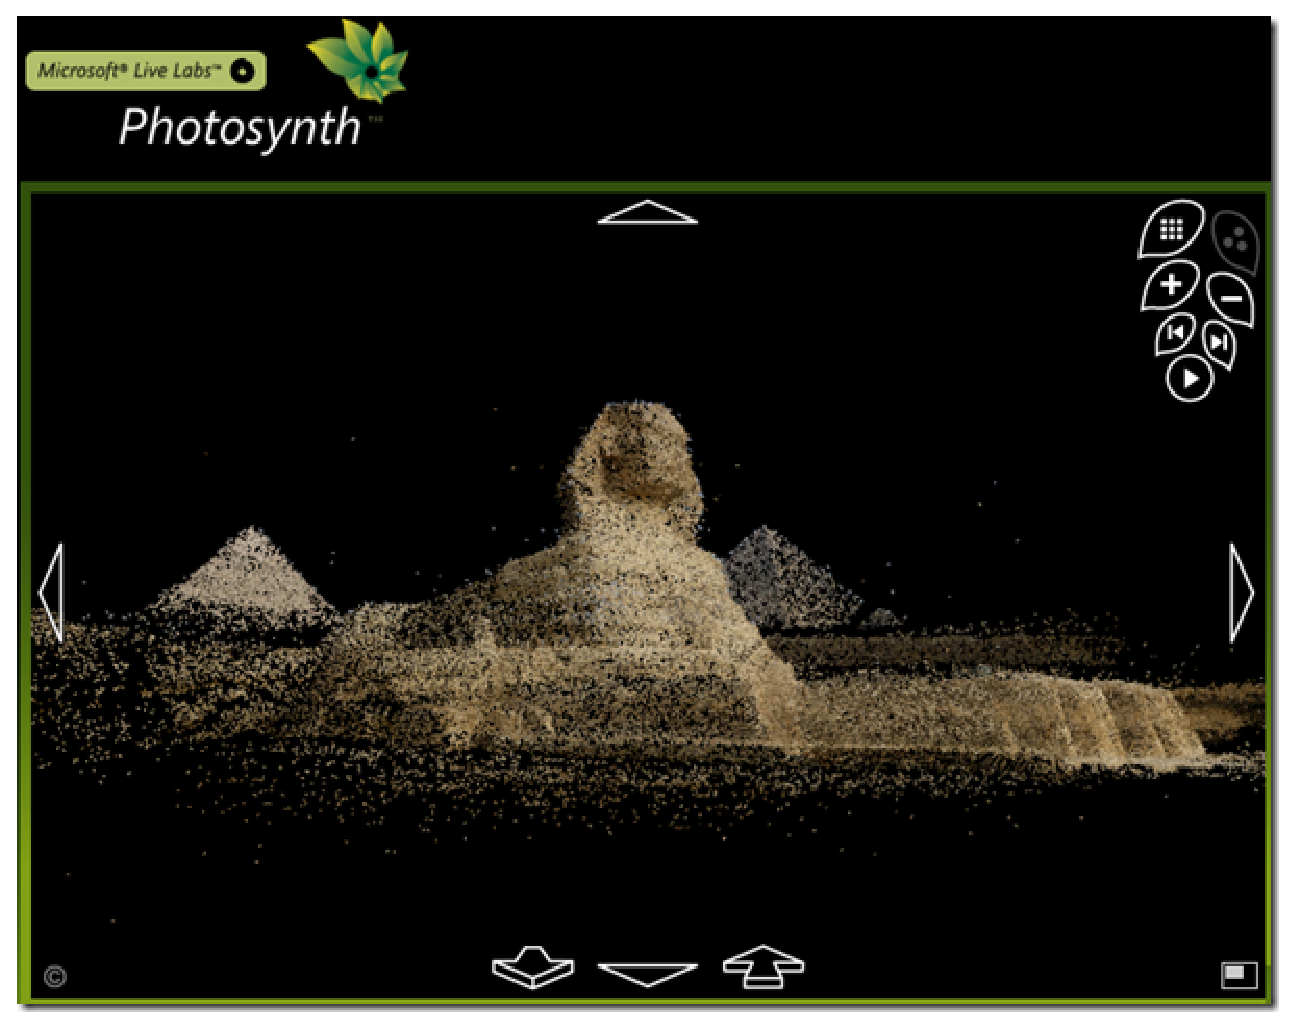
\includegraphics[width=250px]{photosynth}
  \end{center}
  \caption{An Egyptian Sphinx, viewed as Photosynth's point cloud \protect \cite**{photosynth}}
  \label{photosynthcloud}
\end{figure}

\begin{figure}
  \begin{center}
    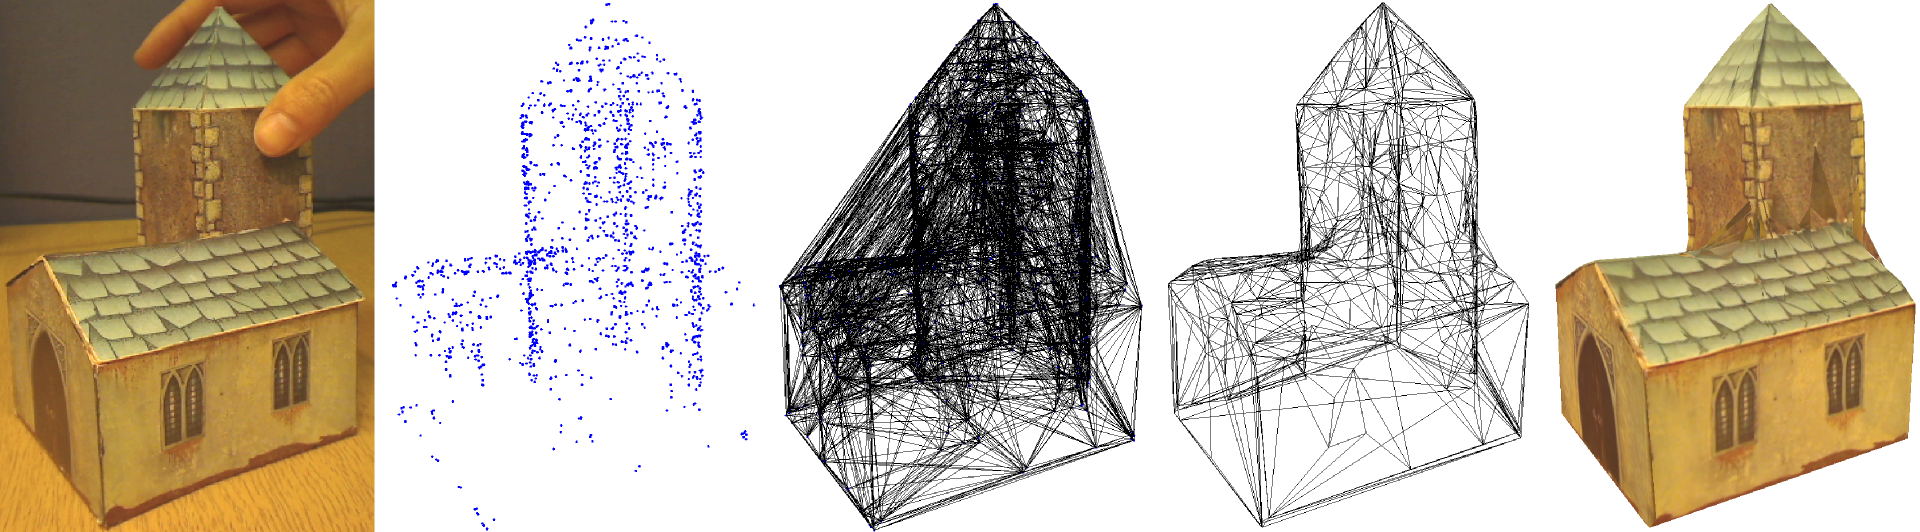
\includegraphics[width=340px]{proforma}
  \end{center}
  \caption{The stages of ProFORMA's automated modelling process \protect \cite**{proforma}}
  \label{proformaeg}
\end{figure}

Alternative approaches go to the other extreme: complete on-line processing of visual data, aiming for an interactive experience \cite**{proforma}. In ProFORMA, the application guides the user as to which areas of the target object it requires further data on, and shows the model in augmented reality as the scanning takes place. The approach taken by Pan is to perform structure-from-motion analysis on the rotating object in order to inform the application as to the angle at which it is viewing the object. From this, it generates and maintains a 3D point-map of the target object. This point map is used as input to a Delaunay Tetrahedralisation \cite**{dtet} process, which is then probabilistically carved to produce a complete mesh. Finally, texture is extracted from the video stream to suit the polygons of this mesh (see Figure~\ref{proformaeg} for an example). However, as we can clearly see in this example (of Qi Pan's own production!), the carving is imperfect; the modelled shape clearly does not quite match the input object, and extra polygons can be seen protruding from the surface of the bell-tower. Should a user wish to clean this up, they would first have to import the data into a 3D modelling package, and then attempt to understand the automated mesh that was generated, in order to alter the polygon geometry and remove these spurious constructions. Furthermore, they would have to manually modify the texture map, since ProFORMA has extracted texture for regions which do not exist in the source shape. 

Debevec et al. \cite**{architecture} produced an interesting, and similar, approach based on a series of static images and minimal user input, tailored primarily for architectural modelling. This required altogether less user input - simply marking edges on the images - but on its relatively limited test domain produced some strong results.

\begin{figure}
  \begin{center}
    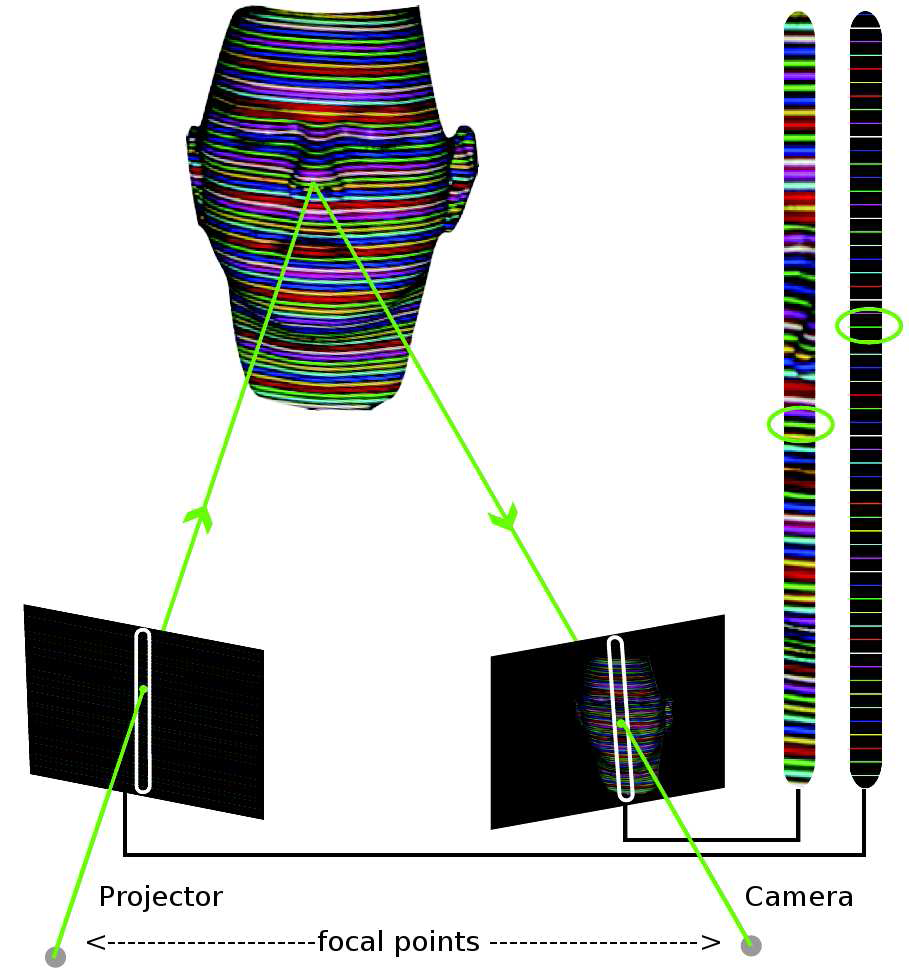
\includegraphics[width=300px]{lightproj}
  \end{center}
  \caption{An example of point projection from the human face using structured light \protect \cite**{lightface}}
  \label{faciallightpoint}
\end{figure}

Another approach that has received recent attention is Structured Light \cite**{structlight}. This entails controlling the lighting of the target object in such a way as to extract 3D data; it requires more equipment and a controlled environment, but can produce interactive performance. Typically, a known pattern of light (potentially changing over time) is projected onto the image, from a fixed source. A single lens may then pick up the way the pattern has fallen on the image, and use this to infer its 3D shape. The suitability of such a process for high-resolution complex modelling has already been shown with 3D facial scanning \cite**{lightface}, as in Figure~\ref{faciallightpoint}. 

\begin{figure}
  \begin{center}
    
\includegraphics[width=340px]{natal}
  \end{center}
  \caption{An example of how Project Natal projects a noisy depth-map onto the human skeleton, \copyright 2009 Microsoft}
  \label{natal}
\end{figure}

This approach is favoured by Microsoft, in their new ``Project Natal" motion camera, which exemplifies structured light's suitability for real-time processing. The Natal system gets around problems inherent in controlling the light in an environment by utilising an infra-red spectrum projection and camera - thereby also preventing visible projected light from dazzling the user. However, such an approach offers insufficient resolution for full 3D reconstruction; Natal extracts a depth map from the scene, and is primarily focused on using this for skeletal mapping and recognition (see Figure~\ref{natal}). Other structured light solutions may be more suitable for the problem described here, however the extra hardware and controlled environment required preclude it as an approach, based on the goals laid out for this system.

\subsection{Surface Reconstruction}

A common aspect of many of these systems is the need to construct a polygon mesh from a point cloud in an automated fashion. This problem is orthogonal to that of extracting the point cloud in the first place; many of these systems could use the same approaches, and differ only in the state-of-the-art at the time of their development. We have already mentioned Delaunay Tetrahedralisation, in the context of ProFORMA. However, this is not the only approach available.

\begin{figure}
  \begin{center}
    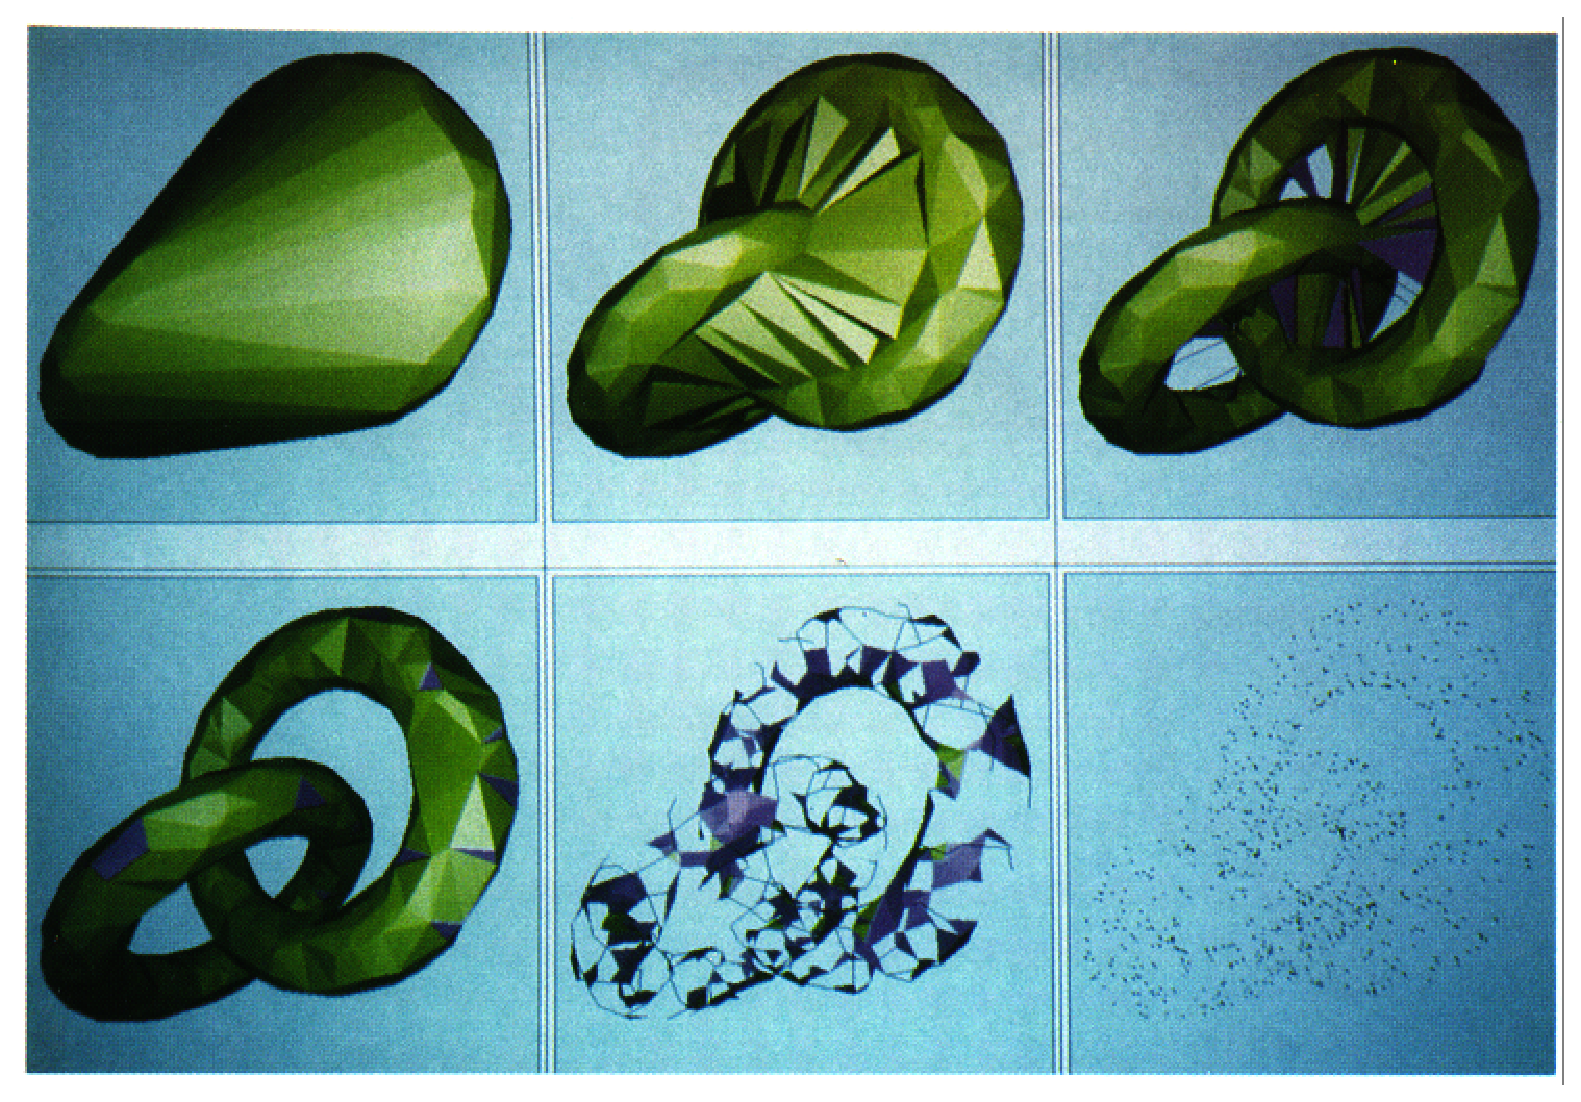
\includegraphics[width=340px]{alphashapes}
  \end{center}
  \caption{A progression of $\alpha$-shapes, with $\alpha$ ranging from $\infty$ to 0 left-to-right and top-to-bottom \protect \cite**{alpha}}
  \label{alphashapes}
\end{figure}

The notion of 3-dimensional $\alpha$-shapes \cite**{alpha} were introduced as an early attempt to fit a manifold onto a cloud of points in 3D space, based on Dalaunay Triangulation (and their dual, Voronoi diagrams). These shapes are a mathematically rigorous generalisation of the convex hull approach \cite**{hull}, with an additional parameter (the eponymous $\alpha$), which defines the range of the family of shapes; as $\alpha$ tends towards 0, the shape tends towards the point cloud. As $\alpha$ tends towards $\infty$, the shape tends towards the convex hull; for values in between, the shape is somewhere between the point cloud and the convex hull - it is not guaranteed that this $\alpha$-shape is fully connected, or necessarily convex, as the convex hull must be. See Figure~\ref{alphashapes} for an example of this in two disconnected tori.

An alternate approach is that of implicit surface reconstruction \cite**{unorgsurf,surface}, in which the surface is estimated as a \textit{simplicial surface} (a linear surface with triangular faces) based on the signed distance between it and the points that comprise its cloud. At each point, a tangent plane is defined as a linear approximation to the surface at that point - how to define the orientation of the planes is characterised by the author as one of the most challenging aspects of this approach. This is done by fitting the least-squares best fitting plane to those points in the ``neighbourhood" of the current point, and subsequently flipping planes to ensure that normals for sufficiently geometrically close points are pointing in similar directions. With these tangent planes constructed, the signed distance function can be estimated based on projecting points onto their nearest tangent plane. Finally, Hoppe uses a marching cubes algorithm \cite**{cubes} to trace contours and perform his final surface construction.

\subsection{User-Driven Vision-Augmented Reconstruction}

\begin{figure}
  \begin{center}
    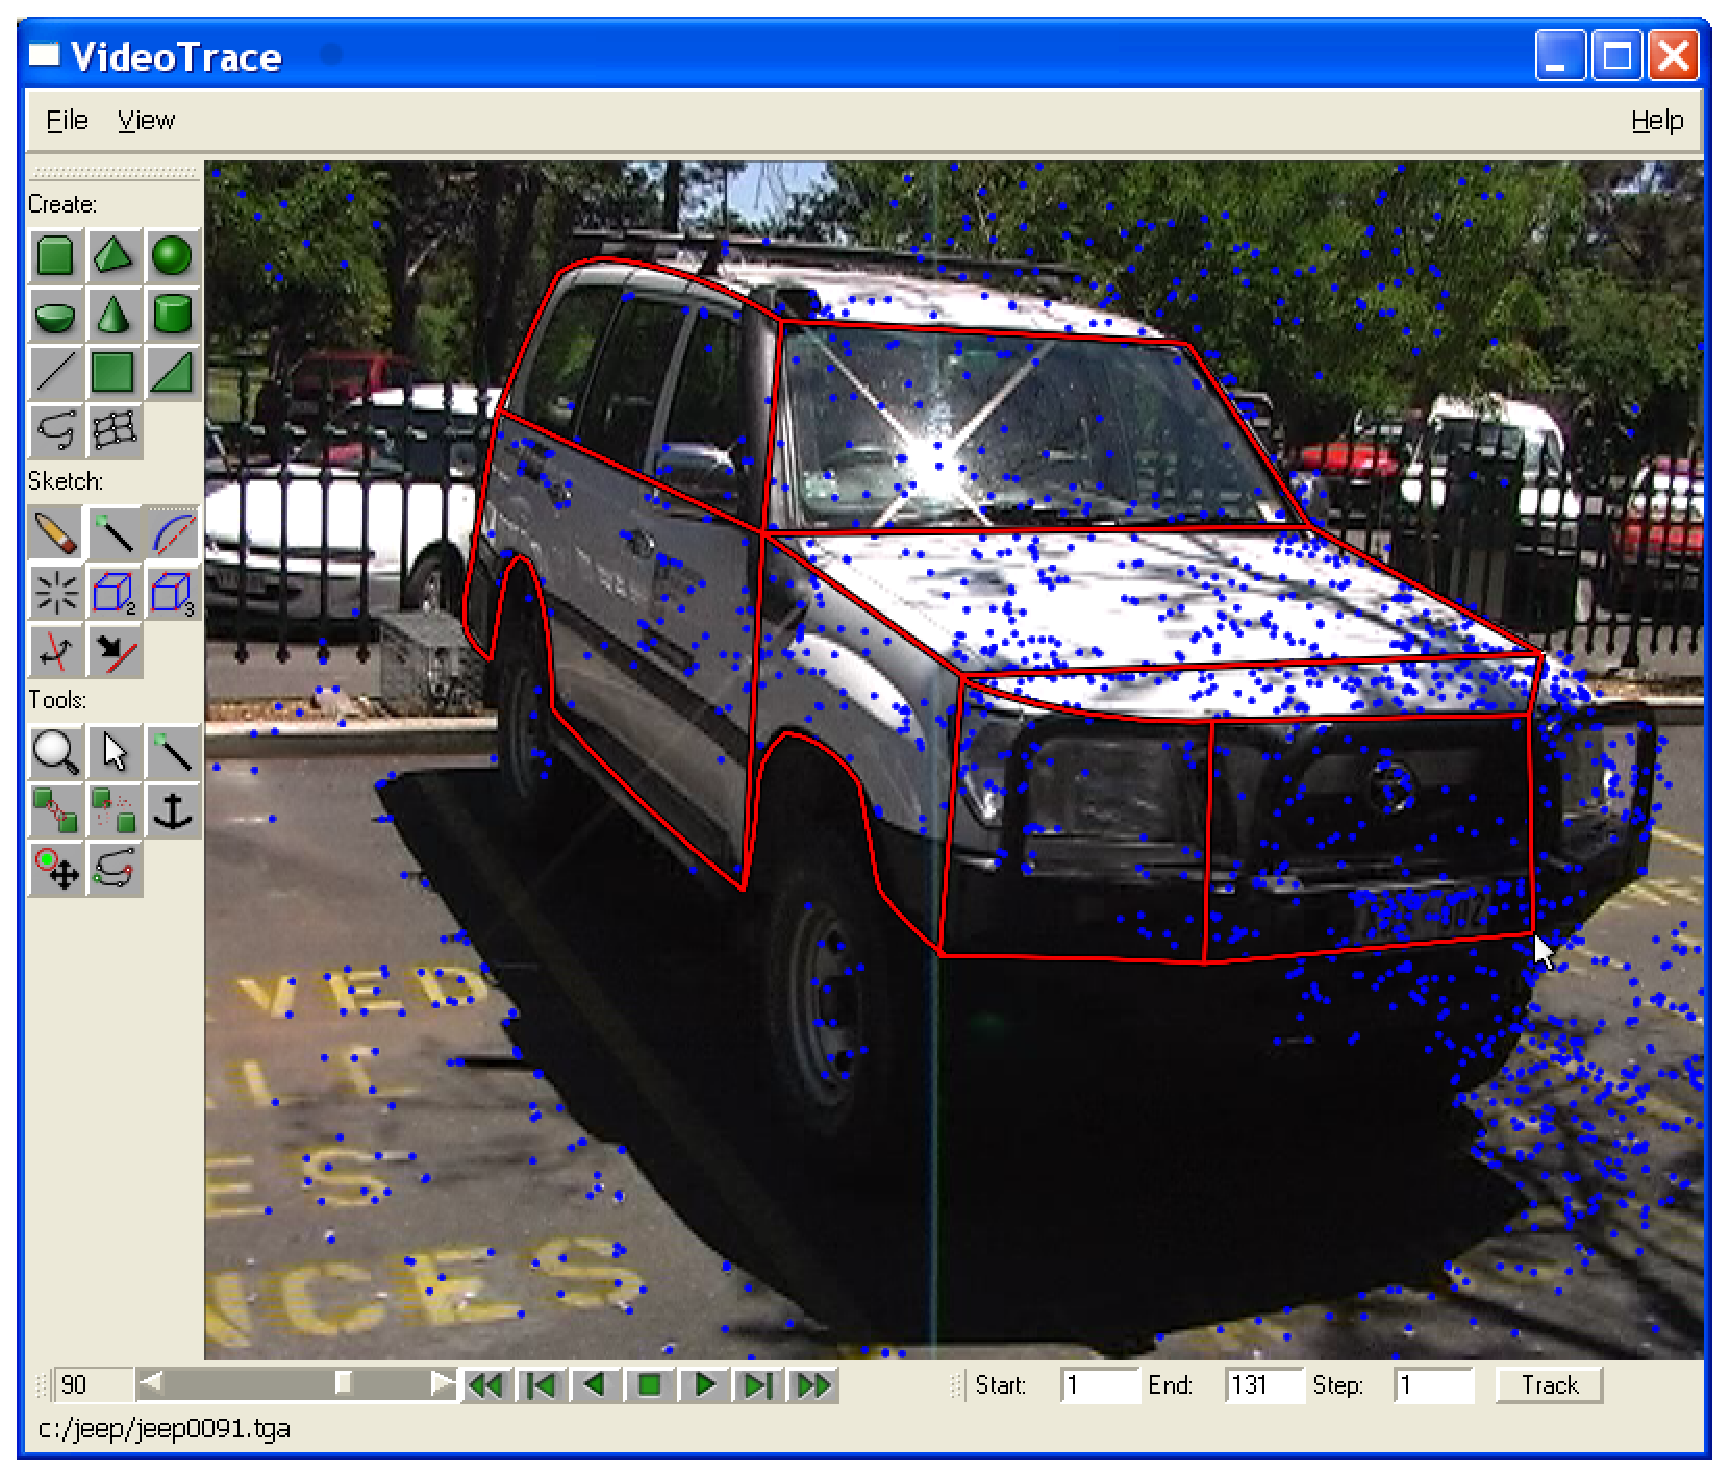
\includegraphics[width=340px]{videotrace}
  \end{center}
  \caption{An example of the VideoTrace User Interface in action \protect \cite**{videotrace}}
  \label{videotraceeg}
\end{figure}

The final approach we will examine is that taken by the likes of VideoTrace \cite**{videotrace}. These approaches recognise the difficulty inherent in producing a solution that will work for ``all of the people, all of the time", and instead focus on creating a toolkit that can be used to trivially craft a model from some video input.

VideoTrace (Figure~\ref{videotraceeg}) uses pre-recorded footage as input to structure from motion analysis, and extracts (in a pre-processing step) a 3D point cloud across the field of view of the camera throughout the sequence. At this time, it caches the results of a number of other computationally expensive vision tasks, such as superpixel segmentation, and thus edgelet delineation (along the boundaries of superpixels). Once this is complete, it presents a highly simplified modelling interface, not entirely dissimilar to SketchUp \cite**{sketchup}. 

VideoTrace uses the vision data already calculated to augment the user's ``tracing" of the video; the user is encouraged to ``scrub" the timeline back and forth, freezing the video on a given frame and then tracing shapes with the given tools (for example straight lines, free-hand drawing, and NURBS curves). As the user does this, VideoTrace snaps these lines to the nearest edgelets, permitting the user's inaccurate interactions to be enhanced by visual structure in the image. VideoTrace offers a suite of tools to help model occluded portions of objects too; for example, by extruding an existing shape or by mirroring geometry along a given plane. All of this processing is informed by visual cues in the image; for example, a user may draw the line of symmetry directly onto a frame of video, and VideoTrace will project that onto its geometry model and construct a fairly accurate mirroring plane. Finally, once the user moves from a given frame of video, VideoTrace processes the traced geometry once more, in order to fix perspective-related inaccuracies; using the continuity of frames to fit the trace to the edgelets in the video, continually enhancing its accuracy.

One obvious pitfall to a VideoTrace-style approach is that one must have enough recorded footage of the object to be modelled a priori; if the available footage doesn't quite show a part of the model, or the texture is occluded or in shadow, new video must be recorded - and this can't be known until one attempts the modelling process. By contrast, interactive systems using live video can show the user in real time what information is lacking, and how they should perhaps tweak their environment to obtain better results.

\subsection{Texture Extraction}

\begin{figure}
  \begin{center}
    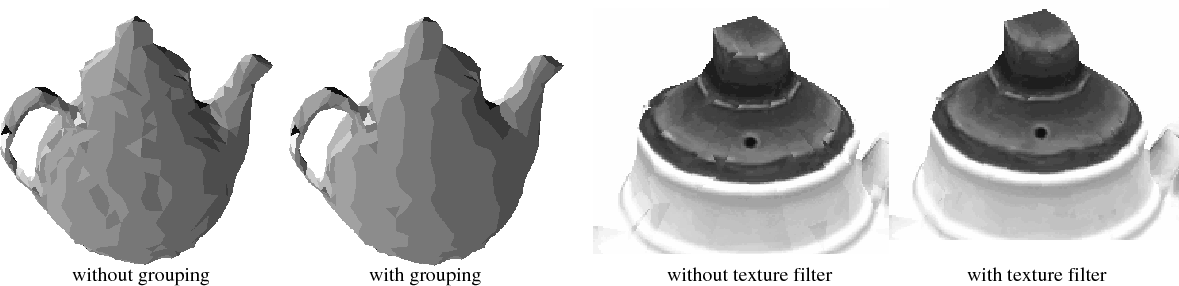
\includegraphics[width=340px]{texture}
  \end{center}
  \caption{A comparison of the various stages of multi-view texture extraction \protect \cite**{texmultiview}}
  \label{texture}
\end{figure}

The final key aspect of these approaches we have not studied in detail is the problem of extracting texture from the input video, and mapping that onto the output geometry. There are a number of elements to this; selection of video frames for texture, compensation for lens distortion and projection of the texture into 2D space, and mapping of this texture onto the generated model such that it forms a contiguous view. A popular technique is to use texture from multiple camera views \cite**{texmultiview} in order to minimise distortions at the boundaries. The approach outlined by Niem and Broszio requires calibration of the camera \cite**{camcalib} in order to remove distortion and reduce aberrations in the input image due to lens shape. It assigns triangles on the surface of the mesh a camera image (selected according to best resolution). Groups of triangles which are textured by the same image (within some tolerance) are then considered to be \textit{surface regions}. These regions are refined so as to group them together as much as possible, reducing the number of region boundaries. Finally, it filters textures at the boundaries by linearly interpolating the texture from one view to the other across the boundary edge. The result is a smoothly varying texture over the surface of the shape; however, it does necessitate choosing sub-optimal video frames for some polygons in the texture-map. The end result of this is a texture map which requires less space to store, and varies smoothly, and thus the trade-off is probably acceptable. Niem and Broszio also describe a technique for synthesising texture for polygons which lack information, by reflecting texture from adjacent regions and blending the results.

The approach taken by Debevec et al. (1996, discussed earlier) sidesteps the issues around perspective quite neatly; the interactive output of their system dynamically selected the texture frame to use based on the current position of the camera. Their approach uses a similar blend technique at polygon boundaries, to reduce rendering artefacts. What is not made immediately clear is how this technique handles a smoothly changing camera; whether it sticks with what is potentially a later non-ideal texture, blends between two target textures smoothly (the problem of knowing which texture to blend \textit{to} seems non-trivial, as it involves predicting the user's interactions), or simply ``jumps" from one texture frame to another at some point in the interaction is not made clear.

\begin{figure}
  \begin{center}
    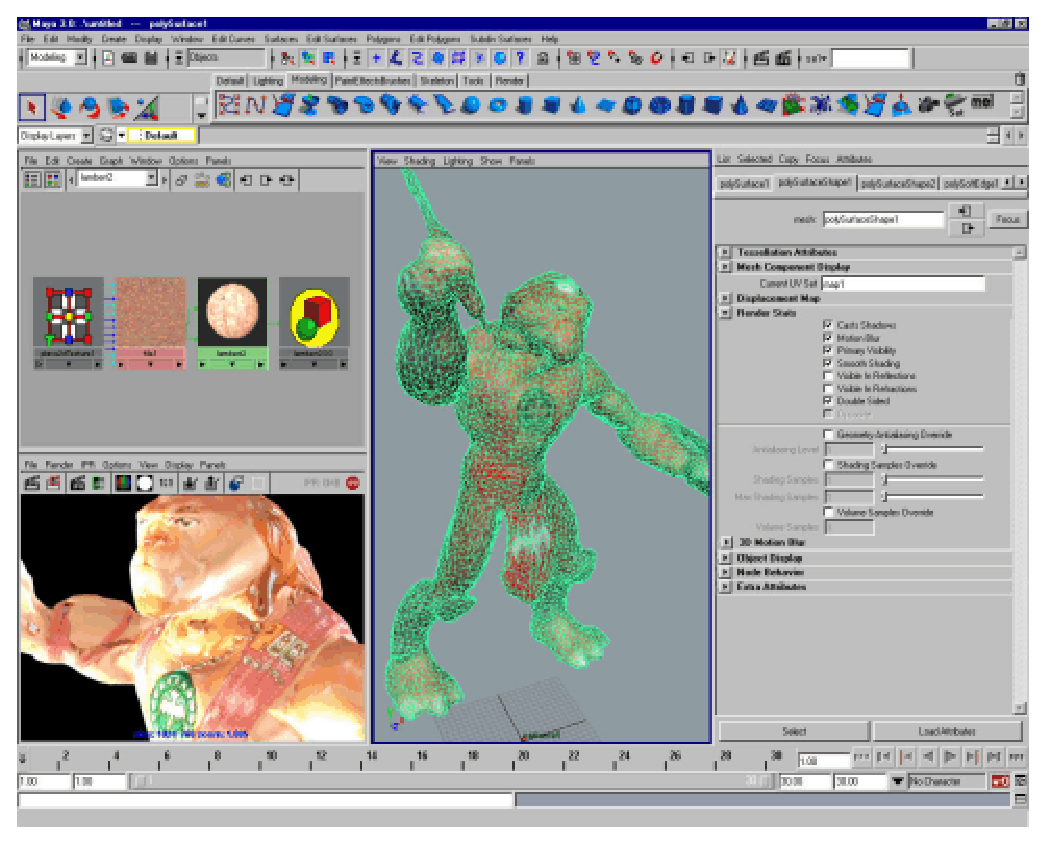
\includegraphics[width=340px]{maya}
  \end{center}
  \caption{An example of Maya's complex user interface (autodesk.com, 2009)}
  \label{maya}
\end{figure}

\clearpage

\section{Approach}
\subsection{Overview}

\begin{wrapfigure}{r}{80pt}
  \vspace{-20pt}
  \begin{center}
    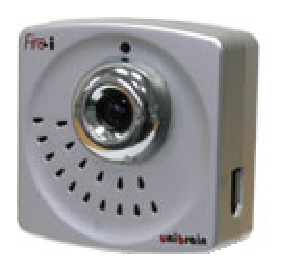
\includegraphics[width=80pt]{firei}
  \end{center}
  \caption{The Unibrain Fire-i\texttrademark}
  \label{firei}
\end{wrapfigure}

Broadly speaking, the approach described herein is to carefully delineate responsibilities between human and machine, so as to make the best possible use of their own varieties of intelligence. For example, heavy \textit{mathematical} reconstruction is an ideal problem domain for a computer; whereas more \textit{interpretive} problems are better solved by the human. The goal of this system is to minimise the complexity of user input (in particular when compared to the likes of Autodesk Maya, Figure~\ref{maya}) by augmenting it with vision technologies. The primary input device is to be a single-lensed commodity webcam, such as the Unibrain Fire-i\texttrademark ~seen in Figure~\ref{firei}.

The goal of the system is to permit the user to move the webcam in space around the object they wish to ``scan", and identify key features to the scanner. Throughout this process, the model created will be updated and continually shown as an augmented reality overlay, so that the user may easily tweak the result and examine its accuracy; this continual feedback loop is required to make the most of the interactivity of the system.

\subsection{Ego-Motion Recovery}
The first problem to be considered in relation to this solution is that of working out where in space the camera is located, and directed, at any given time. Some augmented reality systems, such as Layar, do this by using positioning sensors like GPS in tandem with a magnetometer for orientation. This is a relatively simple way of performing approximate localisation, however the problem of scale rapidly arises; if you desire a resolution of greater than approximately one meter, GPS will quickly fail you. Thus, whilst well suited to (for example) modelling the layout of a whole city, it is less suitable for a user wishing to record a detailed scan of an object on their desk. 3rd party \textit{local} positioning systems operate on a similar principle to GPS, and can provide much greater resolution over small areas. However, they are expensive and seem an unnecessary extra burden for the user to own and maintain. Ideally, the ego-motion recovery problem should be solved without the application of further hardware.

Systems like VideoTrace \cite**{videotrace} are able to make use of processor-intensive offline tracking applications  to perform camera motion recovery - in the case of VideoTrace, the Voodoo Camera Tracker \cite**{voodoo}. These are commonly used in the visual effects industry as well, and thus much effort has gone into research and development on these. They tend to produce excellent and smooth results, even to the extent of being able to automatically fix operator-induced visual defects such as camera shake. However, their processing is designed for batch runs on high-performance machines; they are wholly insuitable to a real-time processing application.

To this end, a number of computer vision researchers have worked on solving the problem of real-time \textit{monocular SLAM}; \textit{S}imultaneous \textit{L}ocalisation \textit{A}nd \textit{M}apping using a single camera lens, with high enough throughput to be used as part of a larger real-time system \cite**{slam}. In essence, a SLAM system works by estimating the movement of the camera between frames based on the motion of the intersection-set of detected feature points in each frame. This approach can produce very accurate results, assuming non-degenerate camera motion. There are instances in which a SLAM-based system can get ``confused", however; it is important that the localiser can detect these cases and re-localise based on the presented frame

\begin{figure}
  \begin{center}
    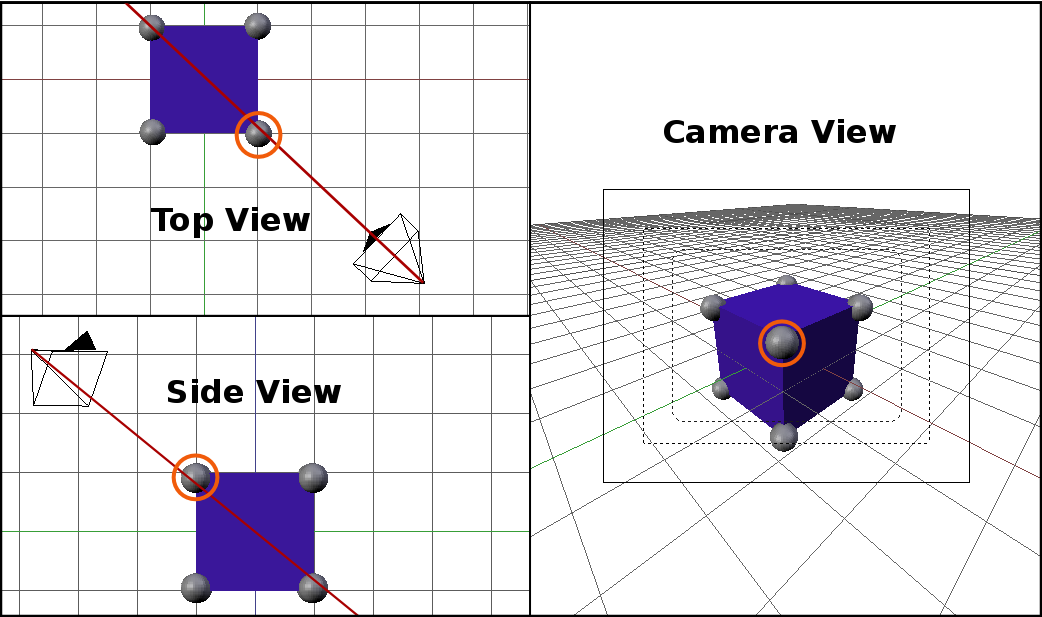
\includegraphics[width=340px]{cameraaim}
  \end{center}
  \caption{An example of the look-vector of the camera aiming towards a set of candidate feature points (marked as spheres), with the closest to that vector ringed}
  \label{lookvec}
\end{figure}

A recent development on existing SLAM approaches is PTAM; \textit{P}arallel \textit{T}racking \textit{A}nd \textit{M}apping \cite**{ptam}. PTAM improves the robustness of SLAM by using a faster approach to motion estimation, thus allowing it to consider far more points in a given iteration of recognition. It can maintain its 3D point-map in a separate thread to the actual motion processing, further reducing the overhead in the tracking thread - making excellent use of common multi-core processing systems available in desktop and laptop computers today. PTAM requires a stereo initialisation at the start, but once this has been processed it will provide a reliable transformation to describe the translation and orientation of the camera in 3D space, relative to an arbitrary zero-point, on an arbitrary scale (both of which are constructed relative to the position and motion of the camera during stereo initialisation). As an added benefit, PTAM maintains a map of the features it recognises in 3D-space. It is highly challenging, given only the position and orientation of the camera, to determine precisely what point in space the user is attempting to point to; there are insufficient bounds on the problem, rendering the system with an infinite vector of possible points. This PTAM point-map can be used to augment such decisions, by deciding which point in the map is closest to the camera's look-vector (see Figure~\ref{lookvec}).

PTAM (as with many SLAM systems) works best with camera lenses exhibiting a wide field-of-view; in this way, it can gather even more points with which to localise. However, this does mean that the images provided to the processing system are distorted by the wide angle lens. In order to account for this, PTAM requires a one-time camera calibration process, which feeds the parameters on its ATAN-Camera model \cite**{atancam}. It is therefore important that, when considering the user interface, this distortion is also considered.

\subsection{User Interface}
As already discussed, the primary user input is to be a simple webcam. This device is to be augmented with a maximum of two other digital inputs (i.e. buttons). These inputs could be positioned on the camera itself - indeed, some cameras already have these. However, in the interests of the most generally usable solution possible, these inputs will be assumed to be on the keyboard.

It is envisaged that the user would interact with the model on the basis of ``tools"; different processors to operate on the scene. One of these input buttons should interact with the selected tool, whilst the second is used to select the tool the user wishes to make use of. Potential examples of tools might be to move points in space, to bisect an edge, or to delete a given vertex in the model.

Feedback is to be provided to the user on a continuous basis. Using the tracking information from PTAM, as well as its camera calibration data, it is possible to project a 3D render of the current model on top of the current camera frame such that it provides a perspective-correct overlay of the current model on the actual object being modelled. To get this right, it will be best to render the model at each stage relative to the co-ordinate system set up by PTAM, then use OpenGL's projection matrix to project those from 3D-space into camera-space. In this way, the projection may also be accelerated by graphics hardware available on the user's computer. However, the scene will need to be rendered twice; once onto an alpha-channel framebuffer in order to do the projection from world-space into screen-space, and once from that onto the camera frame to take into account camera lens distortion. In this manner, an accurate augmented reality scene will be projected atop the camera's image, permitting the user to visualise and improve their results throughout the modelling process.

\subsection{Modelling}
\label{approachmodel}
The modelling process itself should be as general as possible; models should consist of triangular polygons assembled into a valid 3D model. As far as possible, problems such as degenerate faces, co-occurrent points, isolated vertices, etc should be avoided. It is not \textit{necessary} that the produced model be a closed hull; but it should be \textit{possible} to create such a model with this system. The precise details of the modelling process are open to experiments in user-interface design, however it is expected to be a gradual process. The user should work in one of two ways; either they identify vertices in space, and connect them to make the faces of their model, or they may place ``primitives" in the scene (such as planes, cubes, and the like) and manipulate them to best fit the model. Furthermore, there may be cases where a hybrid approach is needed - the user may construct an initial shape that approximates their model, and then refine it over time to improve its accuracy.

It should be possible for the system to use some of the vision techniques above to improve its results - for example, texture extraction may be fully automated. It is important that any vision techniques that are used do not interfere with the will of the user; it must be possible to override their results. A likely example is that of vertex positioning - augmenting the user's input with information about features in the scene can make the task of placing points in 3D space much easier. However, the user \textit{must} have the option of placing points at features that are not detected by vision algorithms. Another useful example of where vision techniques may enhance the modelling process is in edge-fitting; if the user joins two vertices, and the edge is found to run along an edge in the image, the edge that is created in the model may, perhaps, insert extra points in order to better follow the contours of the image. The precise vision techniques that may be applied should be investigated and evaluated for their validity and utility in their particular use cases.

\clearpage

\section{Implementation}
\subsection{Architecture}
In order to realise the above goals, a carefully planned and executed architecture is of prime importance. Broadly speaking, the system is realised as a collection of plugins in four primary areas, with a shared Model at its core. This vision is outlined in Figure~\ref{archmindmap}; here, the Model is represented as an Environment - lists of points in space, the edges connecting them, along with details of the current camera pose and the like.

\begin{figure}[h]
  \begin{center}
	\scalefont{0.9}
	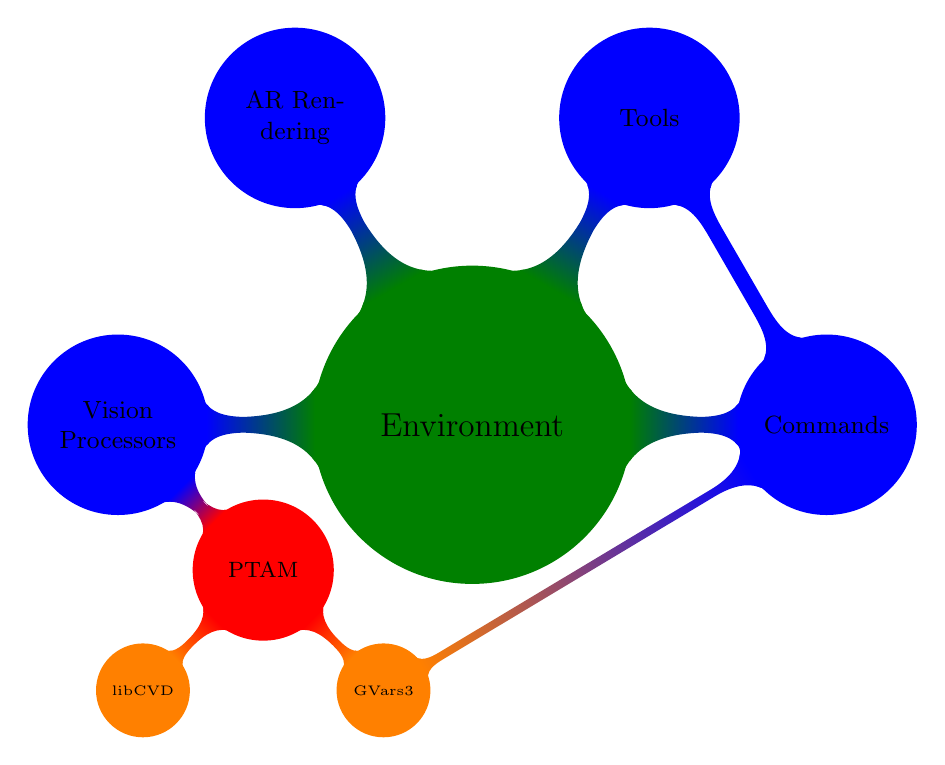
\begin{tikzpicture}[scale=0.9]
  	  \path[mindmap,concept color=green!50!black,text=black]
	    node[concept] {Environment}
	    [clockwise from=180]
	    child[concept color=blue] {
	      node[concept] (proc) {Vision Processors} 
	      [clockwise from=-45]  
	      child[concept color=red] {
	        node [concept] {PTAM}
	        [clockwise from=-45]
	        child[concept color=orange] {
	          node[concept] (gvar) {GVars3} 
	        }
	        child[concept color=orange,sibling angle=90] { 
	          node[concept] (cvd) {libCVD} 
	        }
	      }
	    }  
	    child[concept color=blue] {
	      node[concept] (ren) {AR Rendering}
	    }
	    child[concept color=blue] {
	      node[concept] (tool) {Tools}
	    }
	    child[concept color=blue] {
	      node[concept] (cmd) {Commands}
	    };
	  \path (cmd) to[circle connection bar switch color=from (blue) to (orange)] (gvar);
	  \path (tool) to[circle connection bar switch color=from (blue) to (blue)] (cmd);
	\end{tikzpicture}
	\normalsize
  \end{center}
  \caption{Architectural Vision}
  \label{archmindmap}
\end{figure}

These plugin areas, in blue, are the extension points for the system. In this way, the dependency on PTAM is isolated to the Vision Processors - responsible for any non-interactive ongoing computer vision tasks. ``Commands" in this vision are the direct means of manipulating this model; whether creating new geometry or editing existing polygons. ``Tools", by way of contrast, are the interface between the user's graphical frontend and the rest of the system's internals, interacting with these commands.

The following sections will detail the implementation details of each of these sections in turn, including more formal diagrams as well as details and justification of the design decisions taken along the way. The organisation of these sections reflects the traditional delineation of \textit{Model, View, Controller} exhibited in well architected systems.

\subsection{Model}

\begin{figure}
  \begin{center}
	\scalefont{0.7}
	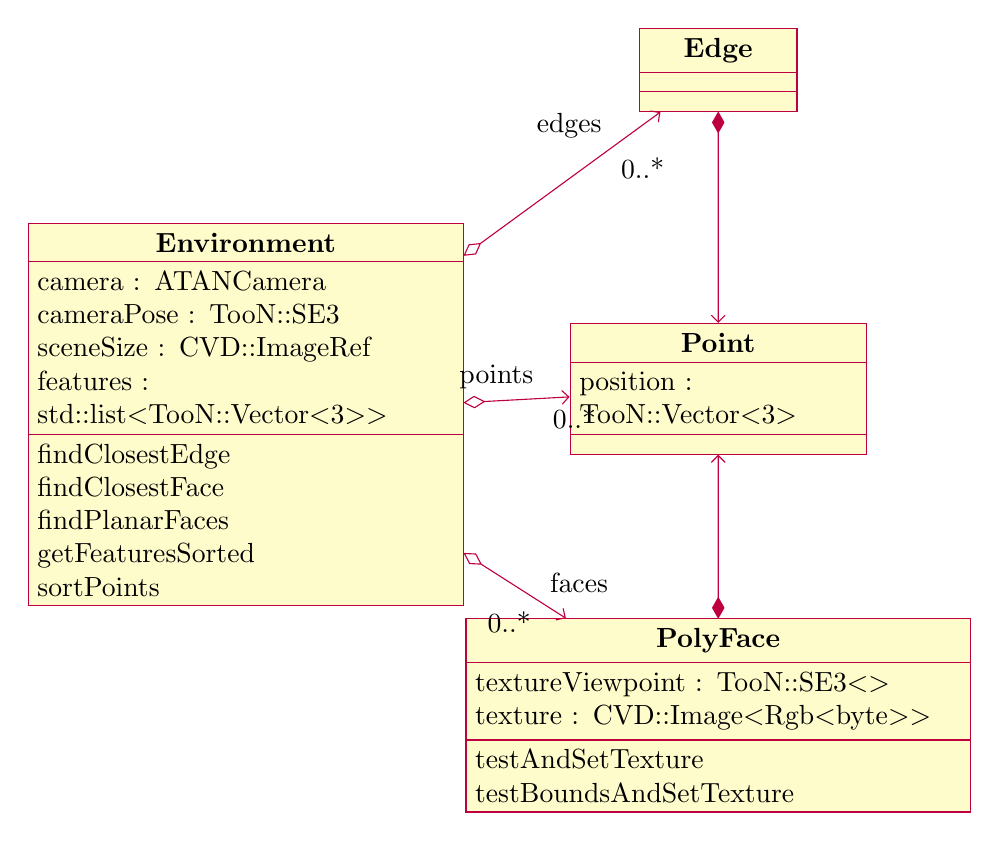
\begin{tikzpicture}[scale=0.75]
	  \begin{class}[text width=150px]{Environment}{0,1.7}
            \attribute{camera : ATANCamera}
	    \attribute{cameraPose : TooN::SE3}
	    \attribute{sceneSize : CVD::ImageRef}
	    \attribute{features : std::list\textless TooN::Vector\textless 3\textgreater\textgreater }
	    
	    \operation{findClosestEdge}
	    \operation{findClosestFace}
	    \operation{findPlanarFaces}
	    \operation{getFeaturesSorted}
	    \operation{sortPoints}
  	  \end{class}

  	  \begin{class}[text width=175px]{PolyFace}{8,-5}
	    \attribute{textureViewpoint : TooN::SE3\textless \textgreater }
	    \attribute{texture : CVD::Image\textless Rgb\textless byte\textgreater \textgreater }
	    
	    \operation{testAndSetTexture}
	    \operation{testBoundsAndSetTexture}
	  \end{class}

	  \begin{class}[text width=100px]{Point}{8,0}
	    \attribute{position : TooN::Vector\textless 3\textgreater}
	  \end{class}

	  \begin{class}[text width=50px]{Edge}{8,5}
	  \end{class}
	  
	  \aggregation{Environment}{faces}{0..*}{PolyFace}
	  \aggregation{Environment}{edges}{0..*}{Edge}
	  \aggregation{Environment}{points}{0..*}{Point}
	  
	  \composition{Edge}{}{}{Point}
	  \composition{PolyFace}{}{}{Point}
	  
	\end{tikzpicture}
	\normalsize
  \end{center}
  \caption{Model Class Diagram}
  \label{modelclasses}
\end{figure}

The aforementioned notion of an \textit{Environment} is carried through from vision to implementation more-or-less verbatim. As seen in Figure~\ref{modelclasses}, there are four classes of note. The main \texttt{Environment} is a single object that is passed to almost all objects in the Scanner system; it contains lists of the \texttt{PolyFace}s, \texttt{Edge}s, and \texttt{Point}s in the system. The classes of \texttt{Edge} and \texttt{Point} are little more than data containers, identifying the lowest level of geometry. Early on it was decided that the core form of geometry in the system should be a triangular polygon; it is the most flexible primitive, and readily maps to the geometry used in 3D modelling packages. Thus, the notion of a \texttt{PolyFace} encodes a triangular polygon as a function of three vertices (\texttt{Point}s from the \texttt{Environment}), with associated texture data. This texture is stored as a full frame from the camera, for later processing. A given \texttt{PolyFace} is capable of deciding whether a given texture frame is better than the currently recorded one, as well as for mapping from the given camera frame to a UV co-ordinate for texture rendering. Finally, the \texttt{PolyFace} may also compute useful quantities, such as the face centre and normal vector, for use in other calculations.

The \texttt{Environment} class is more than just pointers to data, however; it contains a variety of common methods useful for interacting with the model at its lower levels. For example, it contains a list of ``features" extracted by vision algorithms (the details of which are discussed later), along with methods to extract a sorted list of these features based on the current camera position and orientation. Likewise, it can identify which \texttt{PolyFace} or \texttt{Edge} the camera is aimed at, and where on that target the camera is pointed. Other more obvious methods provide interfaces for adding to the model; a method \texttt{addEdge(Point*,Point*)} for example will ensure that the edge is not a duplicate, and automatically construct any new \texttt{PolyFace}s created by this new \texttt{Edge}.

\subsection{Augmented Reality Rendering \& User Experience}

The approach taken for rendering the scene in augmented reality is built on top of that in PTAM's demonstration application. This uses two passes of OpenGL rendering; first, it renders the scene onto a regular framebuffer in memory, and then in a second pass uses the PTAM camera calibration data to distort and render that framebuffer onto the screen. In order to render an Augmented Reality view of the model atop this camera plane, the UFB Linear Frustum Matrix from PTAM is applied as an OpenGL Projection matrix, permitting points in \texttt{Environment}-space to be projected to image-space en masse.

\begin{figure}
  \begin{center}
    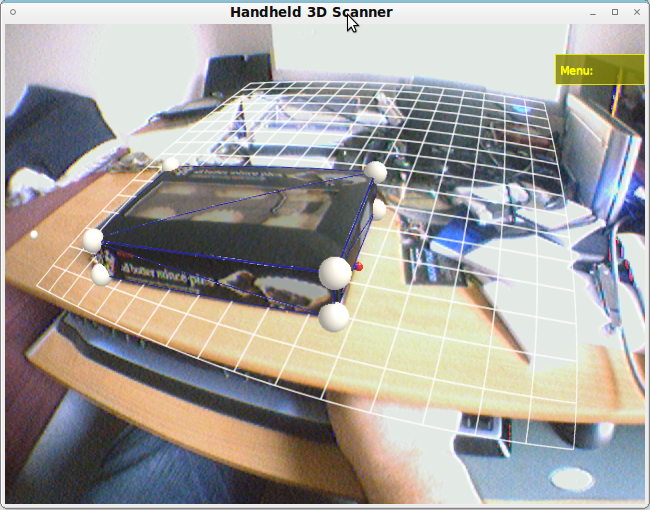
\includegraphics[width=340px]{MincePies}
  \end{center}
  \caption{An early modelling test, showing a textured AR box of mince pies overlaid on the camera plane}
  \label{pies}
\end{figure}

For the purposes of usability, vertices are rendered with an exaggerated size, to facilitate using the camera to ``grab" them. All aspects of rendering are configured using variables in the GVar3 system. For example, a single keypress can be used to toggle rendering of various elements (edges, faces, vertices, camera plane, etc). Further settings include scale settings for things like vertices, or the sensitivity and accuracy of the camera ``pointer" system. Most interaction is done using the camera as a pointer, as described above, seeking feature points around the camera's look-vector; this setting simply adjusts how tolerant this should be of deviation from the precise vector. As seen in Figure~\ref{pies}, the UI is kept to an absolute minimum of clutter (even in early tests such as this). Other usability enhancements present in the system include highlighting of currently targetted objects; these present themselves as orange shading. When creating points it is useful to be able to see the feature points extracted by PTAM's analysis, so the renderer displays the nearest few points, scaled according to their distance from the look-vector of the camera (see Figure~\ref{targets} for an example of this). Usability tweaks like these permit the user to fully predict the behaviour of the system; which face is selected will never be a surprise, and points will always go where the user expects. As this is an interactive modelling system, rather than a fully automated solution, transparency of operation is of the utmost importance.

\begin{figure}
  \begin{center}
    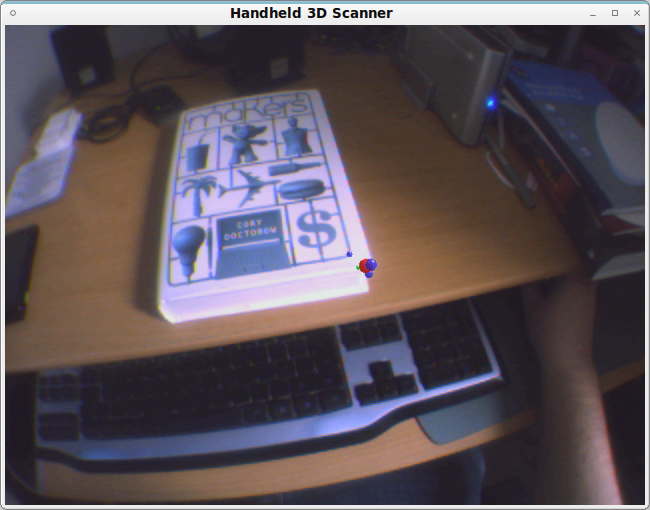
\includegraphics[width=340px]{TargetPoints}
  \end{center}
  \caption{An example of a ``blank canvas" with the nearest target points (blue, red for nearest) to the cursor (green) displayed}
  \label{targets}
\end{figure}

\subsection{Plugins}
\begin{figure}[h]
  \begin{center}
        \scalefont{0.6}
        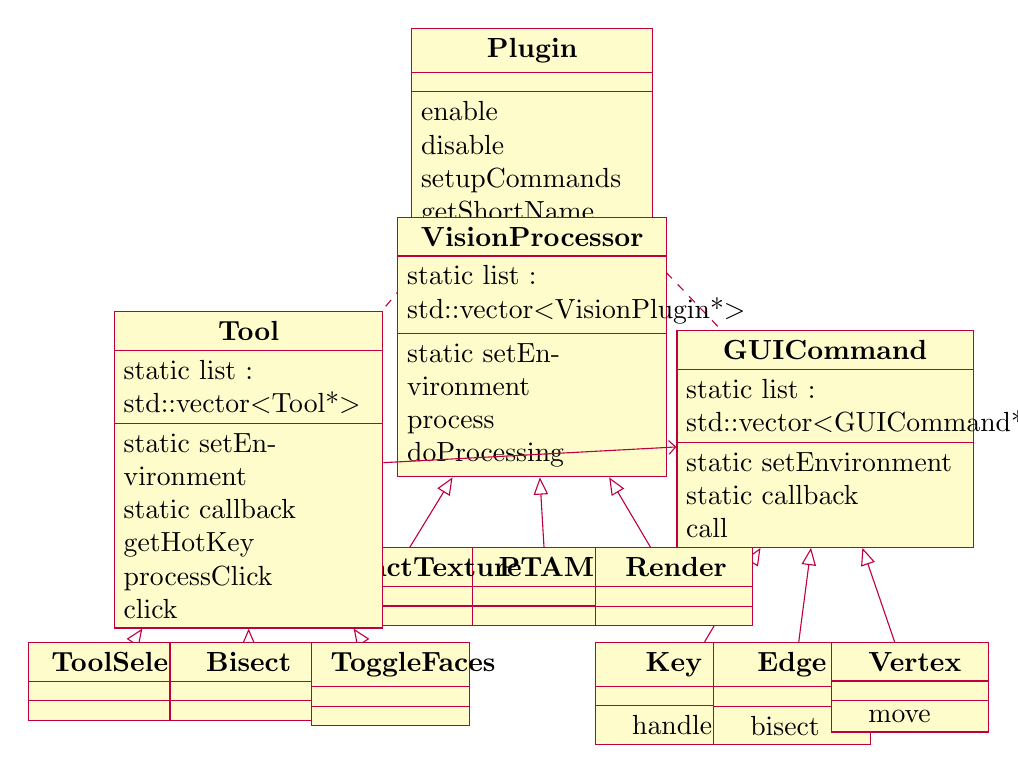
\begin{tikzpicture}[scale=0.6]
          \begin{class}[text width=80px]{Plugin}{0,1}
            \operation{enable}
            \operation{disable}
            \operation{setupCommands}
            \operation{getShortName}
          \end{class}

          \begin{class}[text width=90px]{VisionProcessor}{0,-3}
            \implement{Plugin}
            \attribute{static list : std::vector\textless VisionPlugin*\textgreater}
            \operation{static setEnvironment}
            \operation{process}
            \operation{doProcessing}
          \end{class}

          \begin{class}[text width=40px]{PTAM}{0.3,-10}
            \inherit{VisionProcessor}
          \end{class}

          \begin{class}[text width=35px]{Render}{3,-10}
            \inherit{VisionProcessor}
          \end{class}

          \begin{class}[text width=56px]{ExtractTexture}{-3.1,-10}
            \inherit{VisionProcessor}
          \end{class}


          \begin{class}[text width=100px]{GUICommand}{6.2,-5.4}
            \implement{Plugin}
            \attribute{static list : std::vector\textless GUICommand*\textgreater}
            \operation{static setEnvironment}
            \operation{static callback}
            \operation{call}
          \end{class}

          \begin{class}[text width=30px]{Key}{3,-12}
            \inherit{GUICommand}
            \operation{handle}
          \end{class}

          \begin{class}[text width=30px]{Edge}{5.5,-12}
            \inherit{GUICommand}
            \operation{bisect}
          \end{class}

          \begin{class}[text width=30px]{Vertex}{8,-12}
            \inherit{GUICommand}
            \operation{move}
          \end{class}


          \begin{class}[text width=90px]{Tool}{-6,-5}
            \implement{Plugin}
            \attribute{static list : std::vector\textless Tool*\textgreater}
            \operation{static setEnvironment}
            \operation{static callback}
            \operation{getHotKey}
            \operation{processClick}
            \operation{click}
          \end{class}

          \begin{class}[text width=40px]{ToolSelect}{-9,-12}
            \inherit{Tool}
          \end{class}

          \begin{class}[text width=40px]{Bisect}{-6,-12}
            \inherit{Tool}
          \end{class}

          \begin{class}[text width=43px]{ToggleFaces}{-3,-12}
            \inherit{Tool}
          \end{class}

          \unidirectionalAssociation{Tool}{}{}{GUICommand}

        \end{tikzpicture}
        \normalsize
  \end{center}
  \caption{Plugin Class Diagram}
  \label{pluginclasses}
\end{figure}

Broadly speaking, each \texttt{Plugin} object is a singleton instance of some subclass of the root \texttt{Plugin} type. This core type offers some basic structure as to what makes a ``plugin" in code. All plugins must have a ``short name", which is used to refer to it in configuration. Plugins are also given object-oriented style methods in GVars3, such that a plugin named \textit{``foo"} will automatically have functions registered with GVars3 such as  \texttt{\textit{foo}.enable},  \texttt{\textit{foo}.disable}, or others based on their sub-type. 

As seen in Figure~\ref{pluginclasses}, there are three sub-types in use in the system. \texttt{Tool}s, for example, are used to process the clicks in the user interface (from any hotkey on the keyboard), invoking \texttt{GUICommand}s to perform some action on the \texttt{Environment}. Each \texttt{Tool} specifies which feature type of the image it is concerned with, for user-interface purposes. This may be one of the following;
\begin{itemize}
\item{\textbf{Features} (PTAM's extracted features, closest to the camera's view axis)}
\item{\textbf{Point}}
\item{\textbf{Edge}}
\item\textbf{{Face}}
\item{\textbf{Plane} (A full set of planar faces)}
\end{itemize}

Finally, \texttt{VisionProcessor}s are invoked in a constant processing loop to perform vision tasks, and provide the ``main loop" of the system.

As a coding standard, it is desirable that plugins are as easy to develop as possible. In order to encourage lots of small plugins, rather than monolithic chunks of code, much of the C++ syntactic overhead is removed through the use of preprocessor macros. For example, to declare a \texttt{VisionProcessor} all that is required is an indicator of the type, and optionally any \texttt{protected} variables it should require, thus:

\begin{verbatim}
MK_VISION_PLUGIN( MyVisionAlgorithm, pthread_t workerThread; );

void MyVisionAlgorithm::doProcessing( CVD::Image<CVD::byte>& bw, 
        CVD::Image< CVD::Rgb<CVD::byte> >& rgb ) {
    // My code goes in here
}
\end{verbatim}

\subsubsection{Vision Processors}
\begin{enumerate}
\item{\textbf{cam}: Extracts camera frames from the compiled-in \texttt{VideoSource}, which converts them to their RGB and Black \& White variants for passing on to other vision processors.}
\item{\textbf{ptam}: Invokes the PTAM camera tracking system to track the current video frame. Once tracking is complete, this plugin also records the camera pose into the current \texttt{Environment}, as well as updating the list of features that PTAM is tracking. These features are used by many of the Commands, outlined below.}
\item{\textbf{guiDispatch}: Dispatches any GUI events, and renders the current view. This extends the double-buffered \texttt{GLWindow2} and \texttt{ARDriver} classes from PTAM; in this way, they may reuse the camera calibration for AR projection, as discussed previously, while using our custom \texttt{ARPointRenderer} for actual object rendering.}
\item{\textbf{commandList}: Synchronised plugin to execute commands in the main thread. This uses \texttt{pthread\_mutex} locks to present a thread-safe way of invoking commands from any thread in the system, and ensuring they are executed sequentially, without any interleaving. It offers a static method, \texttt{commandList::exec( string )}, to quickly add a command to the execution list, and then clears this entire list on each call to \texttt{doProcessing}.}
\item{\textbf{textureExtractor}: Test the current texture frame against each polygon in the image to see if it is a better match for texturing than the viewpoint it previously had. Most of the program logic for this is encapsulated within the \texttt{PolyFace} class.}
\item{\textbf{profiler}: Prints out hierarchical profiling timing information to the console. The run-time profiler used throughout the codebase is Shiny \cite{shiny}, a fast and low-overhead C++ profiler. Profiling points can be defined arbitrarily; either as an entire method, or for sub-components, to allow more specific behaviours to be timed. An example of the profiler's output can be seen below:
\begin{verbatim}
call tree               hits       self time      total time
<root>                   1.0      8 us    0%     54 ms  100%
  cam                    1.0     29 ms   53%     29 ms   53%
  ptam                   1.0     13 ms   24%     13 ms   24%
  gui                    1.0      5 ms    9%     13 ms   23%
    DrawStuff            1.0     15 us    0%      8 ms   14%
      DrawPoints         1.0      7 ms   12%      7 ms   12%
      DrawFeatures       1.0     20 us    0%     20 us    0%
      DrawTarget         1.0    842 us    2%    842 us    2%
      DrawPolys          1.0     65 us    0%    200 us    0%
        textureTidyup    9.0     19 us    0%     19 us    0%
        retrieveTexture  9.0     12 us    0%     12 us    0%
        drawTriangles    9.0    104 us    0%    104 us    0%
  commands               1.0     19 us    0%     19 us    0%
  textures               1.0     34 us    0%     34 us    0%
\end{verbatim}
}
\end{enumerate}

\subsubsection{Commands \& Tools}
\label{cmdTools}
\begin{itemize}
\item{\textbf{key.handle}: This is a keypress handler, invoked via GVars3 from the GUI key Dispatch method. It searches the list of tools for any tools which have a matching hotkey to the passed in key, and invokes them; any which are enabled will receive a ``click".}
\item{\textbf{edgelist.dump}, \textbf{pointlist.dump}, \textbf{polylist.dump}: These three debugging commands can be used to dump a list of \texttt{Edge}s, \texttt{Point}s, or \texttt{PolyFace}s to the console, respectively.}
\item{\textbf{text.draw}: This command is designed to be invoked by other commands; it will cause text to be drawn as a ``status update" to the user using OpenGL. This ensures that consistent styling is used, and makes it easy to execute the drawing in the correct thread.}
\item{\textbf{vertex.create}: Creates a \texttt{Point} on the feature closest to the look-vector from the camera. If invoked with parameters, it can create a \texttt{Point} at an arbitrary position (defined by the 3D co-ordinates given in the parameters). The closest point is found by sorting the vector of features with the \texttt{closerVec} function, which works between two vectors thus: 
\\

Given a camera pose $C$, ~let $O ~=~ C_{translation}$
\\

Given therefore that $C_{rotation} = \left[
  \begin{array}{c c c}
    x_1 & x_2 & x_3 \\
    y_1 & y_2 & y_3 \\
    z_1 & z_2 & z_3
  \end{array}\right]$, let $V ~=~ \left[ 
  \begin{array}{c}
    z_1 \\ 
    z_2 \\ 
    z_3 
  \end{array}\right]$.
\\ \\
  
Therefore, with arbitrary vectors $A$ and $B$, $A ~<~ B~$ iff \\$~(A - O ~\times~ A - V) ~~<~~ (B - O ~\times~ B - V)$. \\
}

\item{\textbf{vertex.remove}: This command simply removes the targeted vertex. This vertex is identified from the look-vector using the same \texttt{closerVec} function as described previously.}

\item{\textbf{vertex.move}: This command has two operation modes; the first is a free move, which moves the targeted vertex based on its fixed distance from the camera. The second mode is much the same, but it fixes the motion to be in only one of the three axes; this is simply done using the \texttt{lock} vector, which is 0 when movement in the given axis is to be ignored, and 1 otherwise. The actual movement is performed in a separate \texttt{p\_thread}, and updates the position of the target point as often as the OS' threading model permits according to the following equations:
\\

Given an initial camera pose $C$, and that $C_{rotation} = \left[
  \begin{array}{c c c}
    x_1 & x_2 & x_3 \\
    y_1 & y_2 & y_3 \\
    z_1 & z_2 & z_3
  \end{array}\right]$, the new vertex position at camera pose $C'$ is given by 
\\

$$\displaystyle \left[ 
  \begin{array}{c}
    lock_x \times (C'_x + z'_1 \times \frac{Target_x - C_x}{z_1}) + (1 - lock_x) \times Target_x \\ 
    lock_y \times (C'_y + z'_2 \times \frac{Target_y - C_y}{z_2}) + (1 - lock_y) \times Target_y \\ 
    lock_z \times (C'_z + z'_3 \times \frac{Target_z - C_z}{z_3}) + (1 - lock_z) \times Target_z
  \end{array}\right]$$
}

\item{\textbf{vertex.moveOnAxis}: In order to move a point in more than one axis using the above, the user must either attempt to place it in free space (quite challenging), or move it only one axis at a time - a potentially time consuming exercise. For this reason, a version of vertex movement that locks the motion to a single vector of motion. To do this, the user simply aims the camera down the vector they wish to constrain motion to - for example, by lining up the target point with the location they wish to move it to. When invoked, the tool spawns a new \texttt{p\_thread} which continually updates the position of the target point by taking the closest point of approach of the vector when the tool was invoked, and the camera's current look-vector, thus:
\begin{eqnarray*}
  a &=& axis \cdot axis \\
  b &=& axis \cdot lookVector \\
  c &=& lookVector \cdot lookVector \\
  d &=& axis \cdot (camera_{start} - camera_{current}) \\
  e &=& lookVector \cdot (camera_{start} - camera_{current}) \\
\end{eqnarray*}  Resulting in an updated target point position of:
\begin{eqnarray*}
  TargetPoint &=& camera_{start} + axis \times \frac{a \times e - b \times d}{a \times c - b \times b}
\end{eqnarray*}
}

\item{\textbf{edge.connect}: This simple command is used to identify two vertices, and joins them together automatically with an \texttt{Edge} - automatically avoiding duplication and inserting \texttt{PolyFace}s as edge loops are completed.}

\item{\textbf{edge.remove}: This command is the functional inverse of the connect tool; it disconnects two vertices, destroying any \texttt{PolyFace}s that included these edges.}

\begin{figure}
  \begin{center}
  \subfigure[Split Start]
  {
    \label{edgesplit1}
    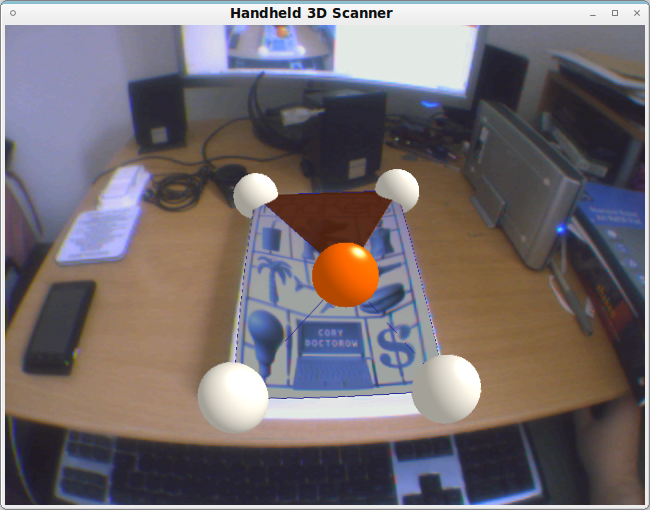
\includegraphics[width=165px]{EdgeSplit1}
  }
  \hspace{-10px}
  \subfigure[Extreme Split Deformation]
  {
    \label{edgesplit2}
    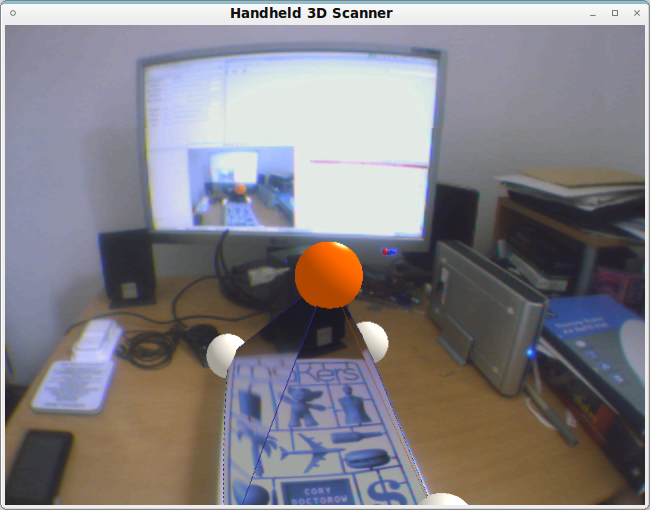
\includegraphics[width=165px]{EdgeSplit2}
  }
  \caption{Behaviour of \texttt{edge.bisect}}
  \label{edgesplit}
  \end{center}
\end{figure}

\item{\textbf{edge.bisect}: The last of the edge manipulation commands, this will insert an extra point on a given edge, splitting any \texttt{PolyFace}s on the way. The edge identification algorithm is the same as for removal; it seeks the point of intersection between the look-vector from the camera and the vector defined by the edge, within some given tolerance. The goal is to minimise $|TargetPoint ~-~ EdgePoint|$ in the following equations;
\\	
        
Let $u ~=~ \left[ 
  \begin{array}{c}
    z_1 \\ 
    z_2 \\ 
    z_3 
  \end{array}\right]$, from the camera rotation, as before, and $v$ be the vector described by the edge in question. Therefore, we can prepare some variables; first, let $p_0$ be the camera's position, and the start point of the current edge be $q_0$. With these definitions in hand,
\begin{eqnarray*}
  w_0 &=& p_0 - q_0 \\
  a &=& u \cdot u \\
  b &=& u \cdot v \\
  c &=& v \cdot v \\
  d &=& u \cdot w_0 \\
  e &=& v \cdot w_0 \\
  Therefore:\\
  EdgePoint &=& q_0 + v \times \frac{a \times e - b \times d}{a \times c - b \times b} \\
  TargetPoint &=& p_0 + u \times \frac{b \times e - c \times d}{a \times c - b \times b}
\end{eqnarray*}

Once we have minimised the above constraint, we ensure that the co-ordinates of $EdgePoint$ lie on the edge, by testing that
\begin{eqnarray*}
0 \leq v \cdot (EdgePoint - q_0) < |v|
\end{eqnarray*}

We therefore know that the target point for the bisected edge is located at $EdgePoint$. The tool for this command also then automatically invokes \textbf{vertex.move}, so that the user may position the point as desired.
}

\item{\textbf{plane.split}: In a similar fashion to \texttt{edge.bisect}, this tool will take a \texttt{PolyFace} and split it at the targeted location. As above, it first finds the targetted face and the point on that face. Next, it removes the targetted \texttt{PolyFace} from the environment, creating a hole in the model. It then places a new vertex in the model at the targetted position, and connects it to the vertices of the old \texttt{PolyFace}, automatically constructing new faces in the process. Finally, it invokes the standard \texttt{vertex.move} tool to permit the user to manipulate the split and tweak its exact location.}

\item{\textbf{plane.move}: With all of the ``primitive" manipulators complete, the next few tools analyse a higher level of geometric structure; namely, permitting the user to treat a collection of faces as a single plane. The constraint for ``planarity" is essentially defined by a tolerance of the angle across an edge; if it is sufficiently close to $0^\circ$, it will consider the attached faces to be part of a single plane. The easiest way to do this, is to consider the angle subtended between the surface normals of these faces, trivially found using the dot-product. The \texttt{Environment} class offers a recursive solution to this problem, which ensures that zero-area faces are ignored (often important when the method is used in the midst of a series of transformations).

The actual movement of this face is handled in a similar fashion to the vertex movement already discussed. A separate worker thread first calculates the face that is currently being ``pointed at", along with the point of intersection between it and the camera's look-vector. To do this, each face is tested first to find its point of intersection: given the camera's look-vector, $z$, a face normal $n$, the camera's position $p_0$ and a point on the face, $p_1$, the shortest vector from the camera to the face can be found as the absolute magnitude of the vector:
\begin{eqnarray*}
  d ~=~ \frac{n \cdot (p_1 - p_0)}{n \cdot z}
\end{eqnarray*}
Finally, a fast bounds-check is used to see if the intersection point with the face's mathematical plane, $p_0 + d$, lies within the bounds of the tested face's actual geometry.

Next, the command's mover thread pre-computes the set of target points to move, and caches their positions before the projection. It then updates positions by calculating the movement the point of intersection on the target face (as in \texttt{vertex.move} and moving all the target points by the same amount.}

\item{\textbf{plane.extrude}: Many common candidates for modelling exhibit symmetrical structures; it thus makes sense for tools to support this mode of modelling. For those objects with lines of symmetry, this extrusion tool will permit the user to:

\begin{enumerate}
 \item{Model a single planar face of the object}
 \item{Create a duplicate plane}
 \item{Automatically connect the vertices of the two planes to form complete polygons}
 \item{Invoke the \texttt{plane.move} tool to manually adjust the distance and direction of extrusion}
\end{enumerate}
}

\item{\textbf{plane.revolve}: Not all symmetry is reflectional; a whole host of objects display rotational symmetry instead. Thus, it is desirable to support this in the modelling as well. To do this, the user need only model half of the rotational face as a plane, and ensure that one of its edges is the axis about which to revolve. Once this is complete, they must simply aim the camera at this axis edge, and invoke this tool to duplicate the original face and rotate it around the axis. The rotation is done with a simple transformation matrix, using a rotation to and from the axis of the revolve, provided by \texttt{TooN::SO3}, thus:
\begin{eqnarray*}
 RotationToAxis \cdot  \left[ 
  \begin{array}{c c c}
    1 & 0 & 0 \\ 
    0 & cos( \theta ) & sin( \theta ) \\ 
    0 & -sin( \theta ) & cos( \theta ) 
  \end{array}\right] \cdot RotationToAxis^{-1}
\end{eqnarray*}
The number of ``steps" to use in this revolve is determined by a configurable GVars3 variable; more steps will increase the quality of the finished geometry, but with it the complexity of the model.}

\item{\textbf{mesh.move}: Commands based on \texttt{mesh.\textit{foo}} manipulate the entire mesh as a whole. This command works in exactly the same manner as the \texttt{vertex.move} command, but applies the vector of movement to \textit{all} vertices of the mesh, instead of just that which is targetted. This command, and \texttt{mesh.scale} (below) are of particular use if larger meshes are to be inserted into the scene - whether through a file import, or by generating primitive shapes. This command will start with the currently targetted point, and pre-compute the closure of all points connected to the target point. In this way, if there are multiple logical meshes in the \texttt{Environment}, only the one which is targetted will be moved.}

\item{\textbf{mesh.scale}: Along with being able to move an entire mesh, it makes sense to use the camera to scale it also; the scale of the axes in world-space are not fixed relative to any given objects, and thus it is unpredictable what size should be used for insertion of an object. This scale command works by scaling the points in the mesh according to the average motion of the target point from its original pose:
\begin{eqnarray*}
  Let p ~=~ Target~start~position \\
  Let q ~=~ Target~projected~position \\
  scaleFactor ~=~ {p_x / q_x + p_y / q_y + p_z / q_z \over 3}  
\end{eqnarray*}

The projection here (to calculate $q$ is done in an identical fashion to \texttt{vertex.move}. Once the $scaleFactor$ has been calculated, it is simply multiplied by the original position of each of the points to scale the mesh - the scale is uniform in all axes. It is valuable to note, also, that the scale tool works only on connected points, in the same fashion as the \texttt{mesh.move} command already discussed.}

\begin{figure}
  \begin{center}
  \subfigure[Low Resolution Mesh]
  {
    \label{lowrescube}
    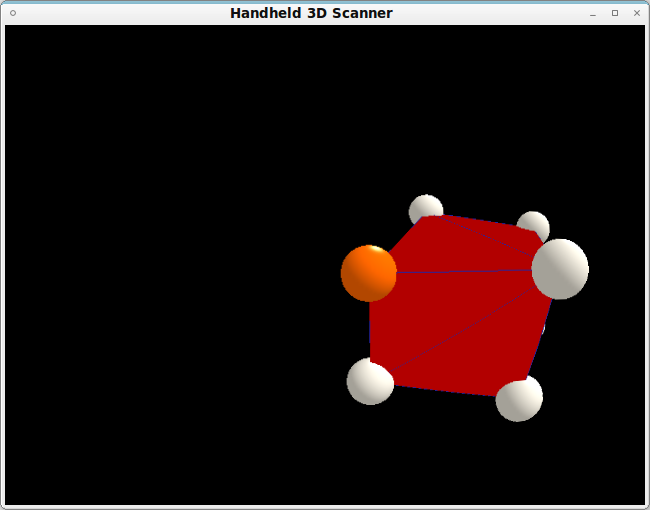
\includegraphics[width=165px]{LowResCube}
  }
  \hspace{-10px}
  \subfigure[Two Iterations of Subdivision]
  {
    \label{subdivcube}
    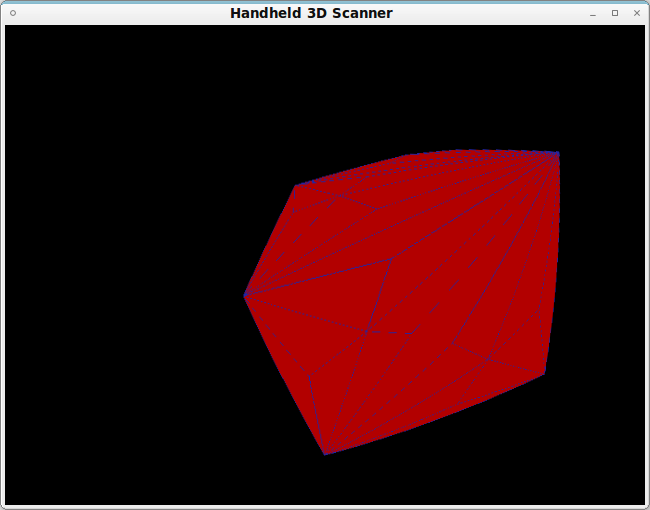
\includegraphics[width=165px]{SubDivCube}
  }
  \caption{Behaviour of \texttt{mesh.subdivide}}
  \label{subdiv}
  \end{center}
\end{figure}

\item{\textbf{mesh.subdivide}: An alternative experiment into ways of improving a mesh's quality, the goal of this command is to improve the resolution of the mesh, smoothing its hard edges, without losing too much detail. The method used is based on Catmull-Clark's mesh subdivision algorithm \cite{catmull}, thus:
\begin{enumerate}
\item{Add new points, on the centre of each face}
\item{Clear all existing \texttt{PolyFace}s in the model}
\item{For each original point in the mesh, calculate the average position of the points connected to it}
\item{Calculate also the average face centre of the faces joined to the current point}
\item{Update the position of the current point as:
\begin{eqnarray*}
 (1 - smoothFactor) \cdot CurrentPos + smoothFactor \cdot \\ \left(FaceAvg + 2 \cdot EdgeAvg + (EdgeCount-3) \cdot \frac{CurrentPos}{EdgeCount}\right)
\end{eqnarray*}
}

\item{Construct new \texttt{PolyFace}s by adding new edges to the model, completing the reconstruction of the model}
\end{enumerate}

The variable $smoothFactor$ above is in fact retrieved from GVars3, where it is called \texttt{catmullSmooth}, to permit the user to configure how much smoothing should be applied in the linear interpolation; as it approaches zero, the positions of the points converge on their original positions. By default, this is kept fairly low so as to introduce some smoothing, but without as much mesh collapse as Catmull-Clark usually causes. This tool can be invoked as many times as desired, to increase the mesh resolution as needed.
}

\begin{figure}
  \begin{center}
  \vspace{-80px}
  \subfigure[Slight Smooth Deformation]
  {
    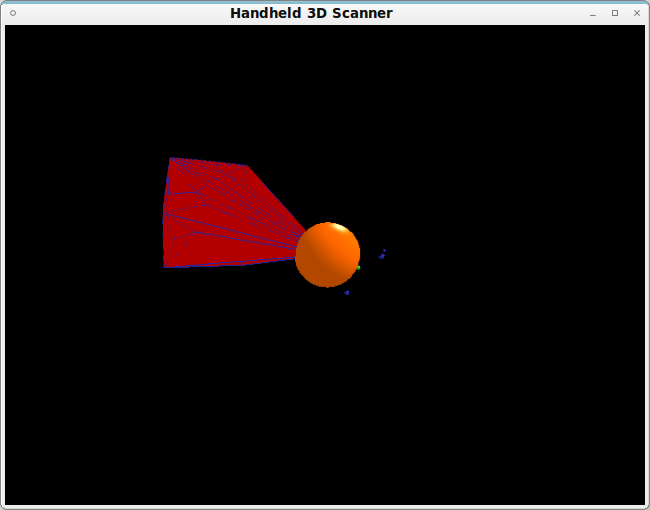
\includegraphics[width=250px]{SmoothDef1}
  }
  \subfigure[Further Smooth Deformation]
  {
    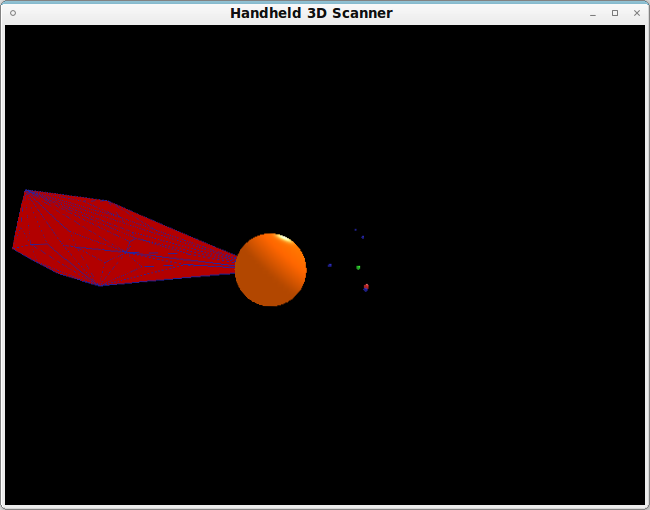
\includegraphics[width=250px]{SmoothDef2}
  }
  \subfigure[Extreme Smooth Deformation]
  {
    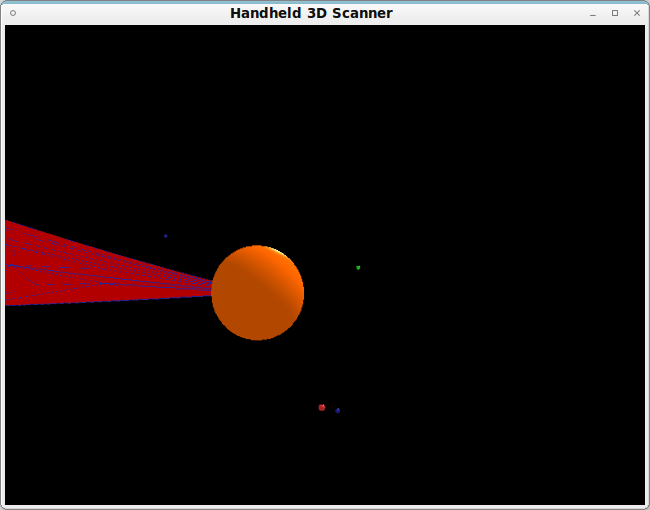
\includegraphics[width=250px]{SmoothDef3}
  }
  \caption{Behaviour of \texttt{mesh.smoothDeform}}
  \label{smoothdef}
  \end{center}
\end{figure}

\item{\textbf{mesh.smoothDeform}: This partner to the \texttt{mesh.subdivide} method is designed to make it easier to manipulate higher resolution models in a smooth fashion; particularly useful when using a high-res model to approximate smooth curves on an objects' faces. To use it, the user simply ``grabs" a point on the mesh, and as they pull it away it will attract the points connected to it, which will in turn attract their neighbours less strongly, et cetera. At its core, this command is very similar to \texttt{vertex.move}, but with an added step on each update; the smooth. GVars3 variables are used to define attraction and inertia factors, while the sterngth of the final pull is calculated as a weighting, $w$, based on the size of the movement of the target point, over the inertia - clamped such that $0 \leq w \leq 1$. The maximum and minimum weights, $w_{max}$ and $w_{min}$ for the other points are then found as the maximum and minimim values of:
\begin{eqnarray*}
 \frac{||TargetPos - PointPos||}{Attraction}
\end{eqnarray*}
Finally, point positions of all points except the target are updated. A per-vertex weight $w_{vtx}$ is calculated, and clamped between $0$ and $1$.
\begin{eqnarray*}
w_{vtx} ~=~ \frac{||TargetPos - PointPos|| \div Attraction - w_{min}}{w_{max} - w_{min}}
\end{eqnarray*}
\begin{eqnarray*}
NewPos ~=~ OldPos ~+~ w \cdot (1 - w_{vtx}) \cdot (TargetPos - PointPos)
\end{eqnarray*}
This smoothing is calculated in real-time, as the user pulls the target point, so that they can see how the deformation alters the entire mesh.
}

\begin{figure}
  \begin{center}
    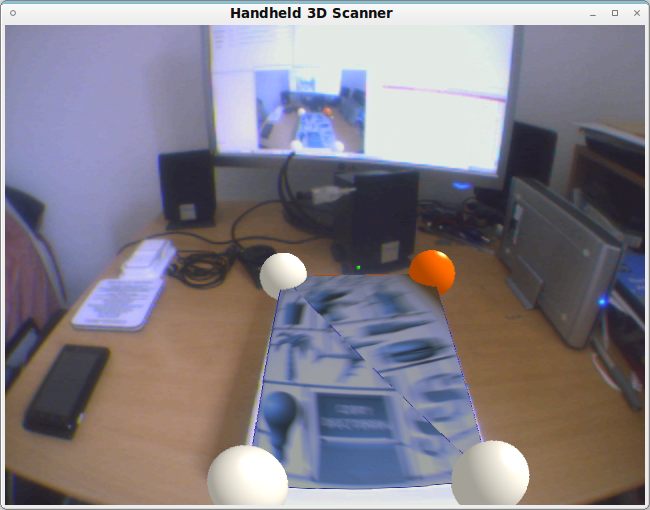
\includegraphics[width=340px]{TextureBlur}
  \end{center}
  \caption{Blurred texture frames captured during fast camera motion}
  \label{camblur}
\end{figure}

\item{\textbf{texture.clear}: As PTAM occasionally and temporarily loses the stability of its tracking, it can capture bad frames of texture - similarly, texture frames can be heavily blurred if the camera was in fast motion when the frame was captured (see Figure~\ref{camblur}). In this event, it is desirable to capture a new texture frame. The simplest way to do this, is simply to clear the existing texture, replacing it with a blank red image, and setting the camera pose for that frame to have been taken from ``infinity". As soon as the camera captures a suitable frame for texturing, which will cover the targetted face, the \texttt{textureExtractor} Vision Processor will update, per its usual operation.}

\begin{figure}
  \begin{center}
  \subfigure[Texture with Discontinuities]
  {
    \label{discont}
    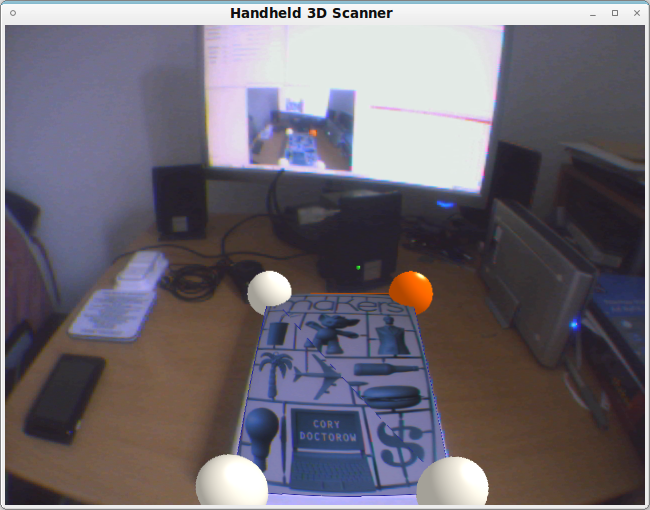
\includegraphics[width=337px]{TextureDiscontinuity}
  }
  \subfigure[Discontinuities removed]
  {
    \label{discontfix}
    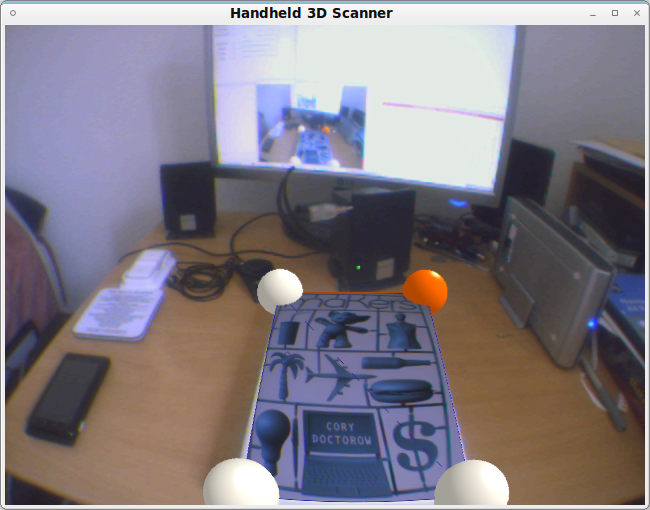
\includegraphics[width=337px]{TextureFixed}
  }
  \caption{Removing texture discontinuity with \texttt{texture.clean}}
  \label{texclean}
  \end{center}
\end{figure}

\item{\textbf{texture.clean}: Often, textures are extracted from camera frames which are very close together, or which could cover more than one \texttt{PolyFace}. Due to the slight inaccuracies of both the PTAM tracking and the texture projection, coupled with the human eye's ability to detect discontinuites in an image, it is desirable to (within reason) choose shared frames of reduced quality, so as to visually improve the result. Furthermore, using fewer frames of video for texturing has the added bonus of reducing file sizes when saving the textures for export. This operation is completed in two passes. The first pass compares the camera pose for each pair of texture frames; if these are within a given tolerance, and the texture frame will cover both polygons, it will be shared between the two faces.

In the second pass, the code examines adjacent pieces ot texture; if the frames are taken from sufficiently similar camera angles, it will choose whichever  image gives the most coverage - if the currently examined face is bounded on at least two sides by the same texture, the angle is within the tolerance, and the texture frame can cover the current face, then the replacement will be performed.}
\item{\textbf{code.save}, \textbf{code.load}: This simple pair of debugging commands demonstrate the power of separating Commands from Tools; they provide a simple way of exporting model geometry, and reloading it later. The save command simply streams a series of primitive commands - only \texttt{vertex.create} and \texttt{edge.connect} are required to reconstruct the model; GVars3 will then load the file later, and the model will be reconstructed. Both commands can take a filename as a parameter, to identify which file to use to save / load (otherwise it will use ``scanner\_model.out", the default filename).}

\begin{figure}
  \begin{center}
    \begin{tabular}{| c | c || c |} \hline
      \textbf{Data Type} & \textbf{Field} & \textbf{Value} \\ \hline
      \texttt{byte} & ID Field Size & 0 \\ \hline
      \texttt{byte} & Colour Map Type & 0 \textit{(none)} \\ \hline
      \texttt{byte} & Image Type & 2 \textit{(RGB)} \\ \hline
      \texttt{byte} & Colour Map Start & 0 \\ \hline
      \texttt{short int} & Size of Colour Map & 0 \\ \hline
      \texttt{byte} & Bits per Pixel in Map & 24 \\ \hline
      \texttt{short int} & X Origin & 0 \\ \hline
      \texttt{short int} & Y Origin & 0 \\ \hline
      \texttt{short int} & Image Width & \texttt{Camera Frame Width} \\ \hline
      \texttt{short int} & Image Height & \texttt{Frame Height $\cdot$ Num Frames} \\ \hline
      \texttt{byte} & Bits per Pixel in Data & 24 \\ \hline
      \texttt{byte} & Image Descriptor Bits & 0 \\  \hline
      \multicolumn{3}{|c|}{\textit{\texttt{B-G-R} bytes of texture data in reverse order follows}} \\
      \multicolumn{3}{|c|}{\textit{\texttt{...}}}
    \end{tabular}
  \end{center}
  \caption{TARGA Image File Format}
  \label{tgaformat}
\end{figure}

\item{\textbf{obj.save}: While the above provides one form of save utility, it does not satisfy the need to load models generated in this tool into any other industry standard tools. In order to do that, the Wavefront OBJ format\cite{objmtl} was selected as the export format of choice. When invoked, this command will save using the specified file's basename. The Wavefront format allows for saving geometry, material data, and texture data as three separate files. As the texture is stored uncompressed, this command will first invoke the \texttt{texture.clean} command above before it saves. 

The reduced set of texture frames are then stored, as a series of consecutive images in a single 24-bit RGB TARGA\cite{targa} file (see Figure~\ref{tgaformat}). The material data is stored in a \texttt{.mtl} file, which is essentially a plain text format defining the ambient, diffuse, and specular components of the named material (fixed at $1$, $1$, and $0$ respectively). It also permits selection of alpha transparency, and the illumination model to be used, along with naming the TGA file to use for texturing. This file is more-or-less the same regardless of the model. For example,

\begin{verbatim}
# Material database for scanner_model.obj
#  Declares a new material called `TextureMapped'
#    containing the link to the TGA texture file,
#    and details of the material properties

newmtl TextureMapped
    Ka 1.000 1.000 1.000  # Ambient reflection
    Kd 1.000 1.000 1.000  # Diffuse reflection
    Ks 0.000 0.000 0.000  # Specular reflection
 
    d 1.0    # Alpha Transparency
    Tr 1.0   #  (some implementations use d, others Tr)
    illum 2  # Illumination model - Diffuse and Specular
    map_Ka scanner_model.tga  # Ambient map
    map_Kd scanner_model.tga  # Diffuse map
     # Currently does not use:
     # map_Ks   -  Specular map
     # map_d    -  Alpha transparency map
     # map_bump -  Bump map
\end{verbatim}

Finally, the \texttt{.obj} file encodes the details of the model's geometry; the set of vertices, their texture co-ordinates, and the vertex normals. The last section of this file links the OBJ geometry to the material file, and applies the texture to the set of face definitions which follow. These definitions are made in such a way as to ensure that the points are connected in an order which will preserve their surface normals - implicit in the OBJ definition. The OBJ file structure is as follows:

\begin{verbatim}
#
# Header indicating how many vertices and faces are encoded
#   in the file, for human interest
#

# Material library links:
  mtllib scanner_model.mtl

# Vertices:
  v 0.112184 -0.549372 0.636787
  v 0.130041 -0.377297 0.638883
  v 0.246977 -0.535198 0.444692
#  etc...

# Texture Co-Ordinates:
  vt 0.424639 0.217299
  vt 0.273666 0.0712889
  vt 0.33988 0.0545356
#  etc...

# Normals (currently one per face):
  vn 0.0824474 -0.892047 0.444359
  vn 0.200107 -0.88881 0.41228
  vn 0.971032 -0.025272 -0.237608
#  etc...

g scanner_model  # Polygon group name
# Faces:
  usemtl TextureMapped   # Load this material from MTL file
  f 9/1/1 35/2/1 33/3/1  # One triple per vertex in the face
  f 9/4/2 39/6/2 35/5/2  # Each triple indicates vertex id,
  f 9/7/3 19/9/3 35/8/3  #   texture coord id, and normal id
#  etc...
\end{verbatim}

\begin{figure}
  \begin{center}
  \subfigure[Importing Model into Blender3d]
  {
    \hspace{-30px}
    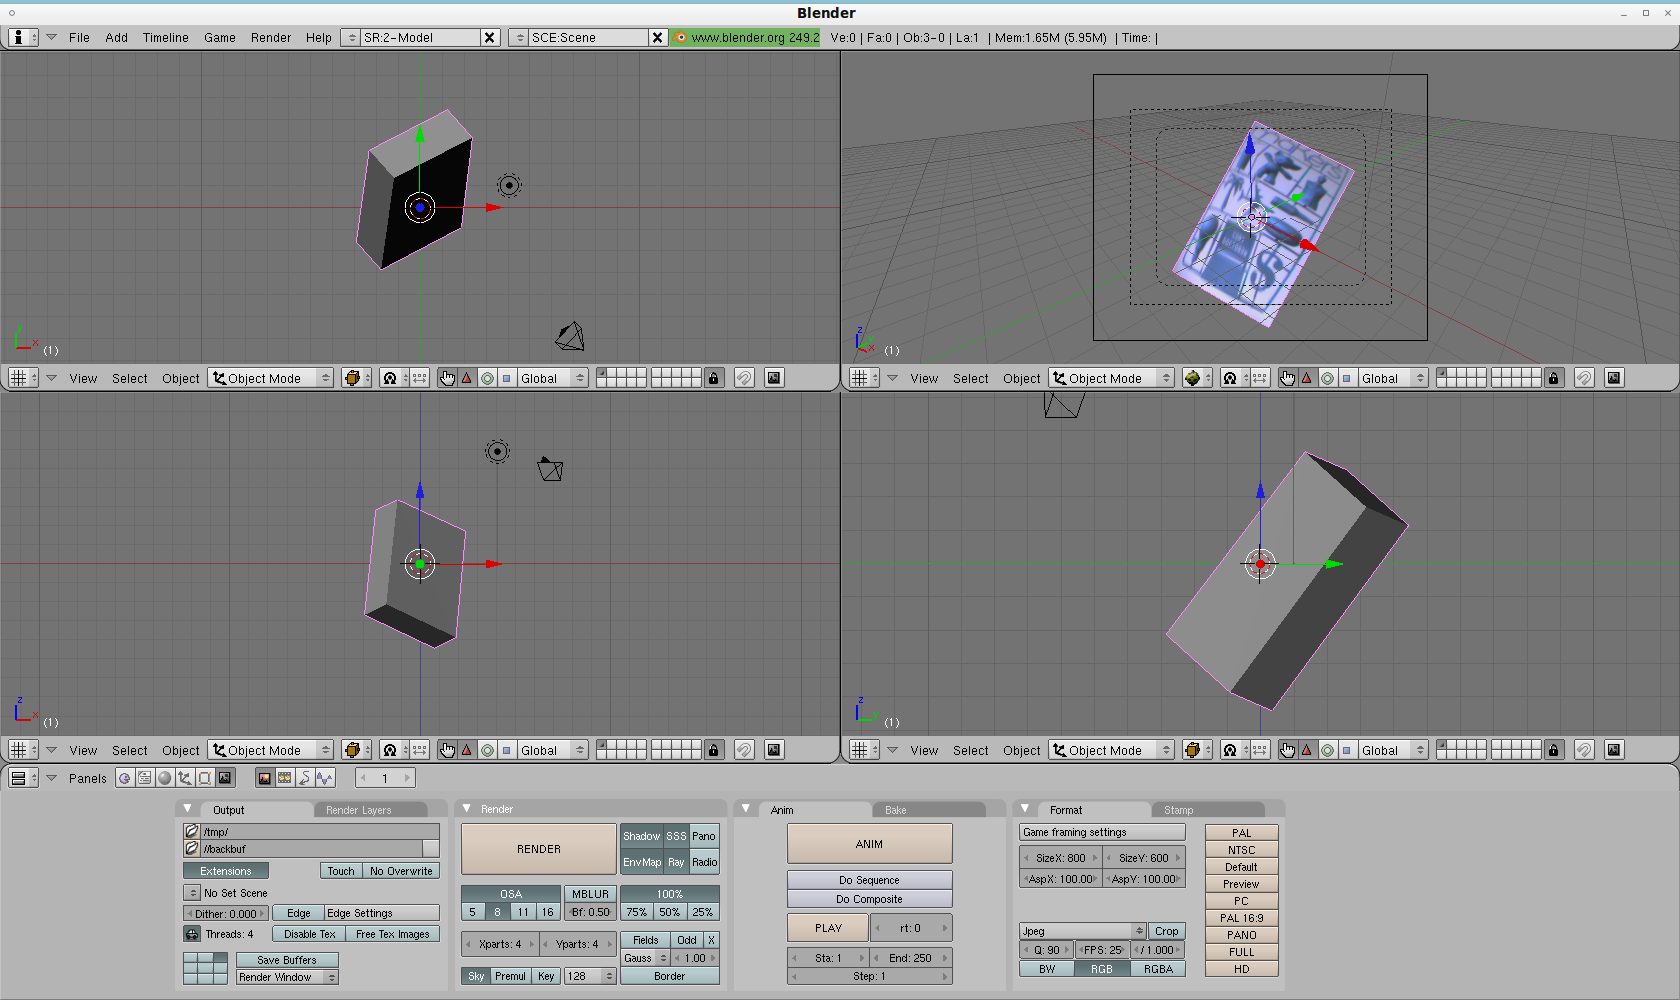
\includegraphics[width=400px]{Blender}
  }
  \subfigure[Rendering with Blender's built-in Renderer]
  {
    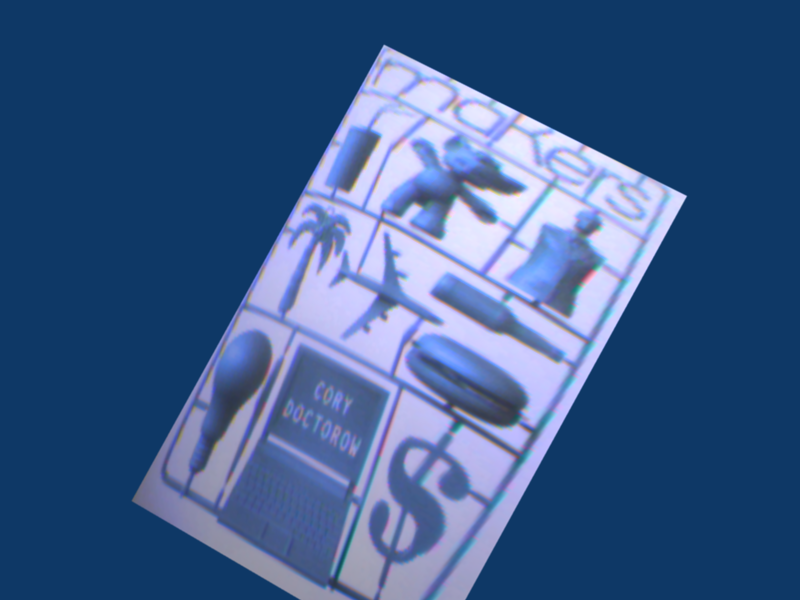
\includegraphics[width=340px]{BlenderRender}
  }
  \end{center}
  \caption{Using the Export feature to load the model into Blender3d}
  \label{blender}
\end{figure}

With all three of these files serialised and linked, most standard modelling tools used in industry today can import without loss of information. An example of this is shown in Figure~\ref{blender}.}

\begin{figure}
  \begin{center}
    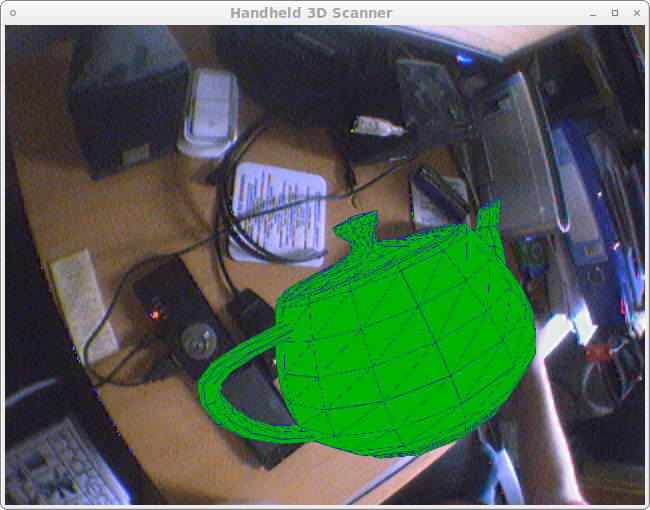
\includegraphics[width=340px]{Teapot}
  \end{center}
  \caption{An example of shaded geometry loaded into the modelling system from an external source}
  \label{load}
\end{figure}

\item{\textbf{obj.load}: Loading of OBJ files is a slightly more complex problem; due to the vast array of options and formats for storing OBJ, MTL, and TGA data the \texttt{obj.load} command will only work with a subset of files. The assumptions it makes are:
\begin{itemize}
\item{Meshes are triangulated (i.e. contain no faces of order \textgreater~3)}
\item{Only one material database has been linked}
\item{Only one material from this database is applied to all faces}
\item{The \textit{diffuse} colour component (\texttt{map\_Kd}) from this material may be applied if no texture data is present}
\item{TARGA images are stored uncompressed, in 24-bit or 32-bit colour (alpha channel ignored)}
\end{itemize}

Any texture data which is loaded from disk for this geometry is stored in a single \texttt{Image\textless Rgb\textless byte\textgreater \textgreater}, which is assigned to a special subclass of \texttt{PolyFace}: \texttt{FixedPolyFace}. This subclass considers its texture to be immutable; the geometry of the loaded model may be changed, but the texture may not under any circumstances. At no point does a \texttt{FixedPolyFace} recalculate its texture UV co-ordinates.
}
\end{itemize}

\subsection{Configuration}
Throughout the implementation, it has been noted that GVars3 variables are used to expose user-configurable parameters. A full list of these can be seen in Appendix~\ref{configparams}. However, for a user to modify them they really need to know what they're looking for; they could type \texttt{gvarlist} in the tool's terminal, but this will list all variables in both PTAM and this system, many of which a user need not concern themselves with. Furthermore, there is no structure to these values, or indication as to how they should be set. Finally, a user may make mistakes when typing a variable, and not realise their mistake until it is too late.

\tikzset{
>=stealth',
  chainel/.style={
    rectangle, 
    rounded corners, 
    draw=black, very thick,
    text width=6em, 
    minimum height=3em, 
    text centered, 
    on chain},
  every join/.style={->, thick,shorten >=1pt},
}
\begin{figure}[h]
  \begin{center}
    \begin{tikzpicture}
      [node distance=.8cm,
       start chain=going right,]
      \node[chainel, join] (sess) {Session};
      \node[chainel, join] (file) {Settings File};
      \node[chainel, join] (code) {Default in Code};
      \node[chainel, join] (code) {C++ Empty Constructor};
  \end{tikzpicture}
  \end{center}
  \caption{Precedence of Configuration Variable Value Sources}
  \label{configprecedence}
\end{figure}

There are two further ways for a user to configure the system; in the settings file, \texttt{settings.cfg}, and through a graphical user interface. There is a well-defined order of precedence to these variables; illustrated in Figure~\ref{configprecedence}. The settings file is pre-populated prior to distribution with all of the default values in the system, and is loaded with the system to set any default values, as if they were typed in on the system's command interface. This means that any plugins can be disabled in the configuration file, also (such as the \texttt{profiler} discussed previously).

The configuration GUI divides up the configuration options by area; Processors, Commands, and ARRendering. The controls either take the form of a toggle button, or a slider, based on the data type of the value. The Processors section also includes buttons to enable and disable various \texttt{VisionProcessor}s. By default, these include:

\begin{enumerate}
\item{PTAM Tracking}
\item{Texture Extraction}
\item{Periodic Texture Cleaning (\texttt{texture.clean})}
\item{Profiler (by disabling this calculation of results does not occur, nor their output to stdout)}
\item{FPS Display}
\end{enumerate}

\begin{figure}
  \begin{center}
    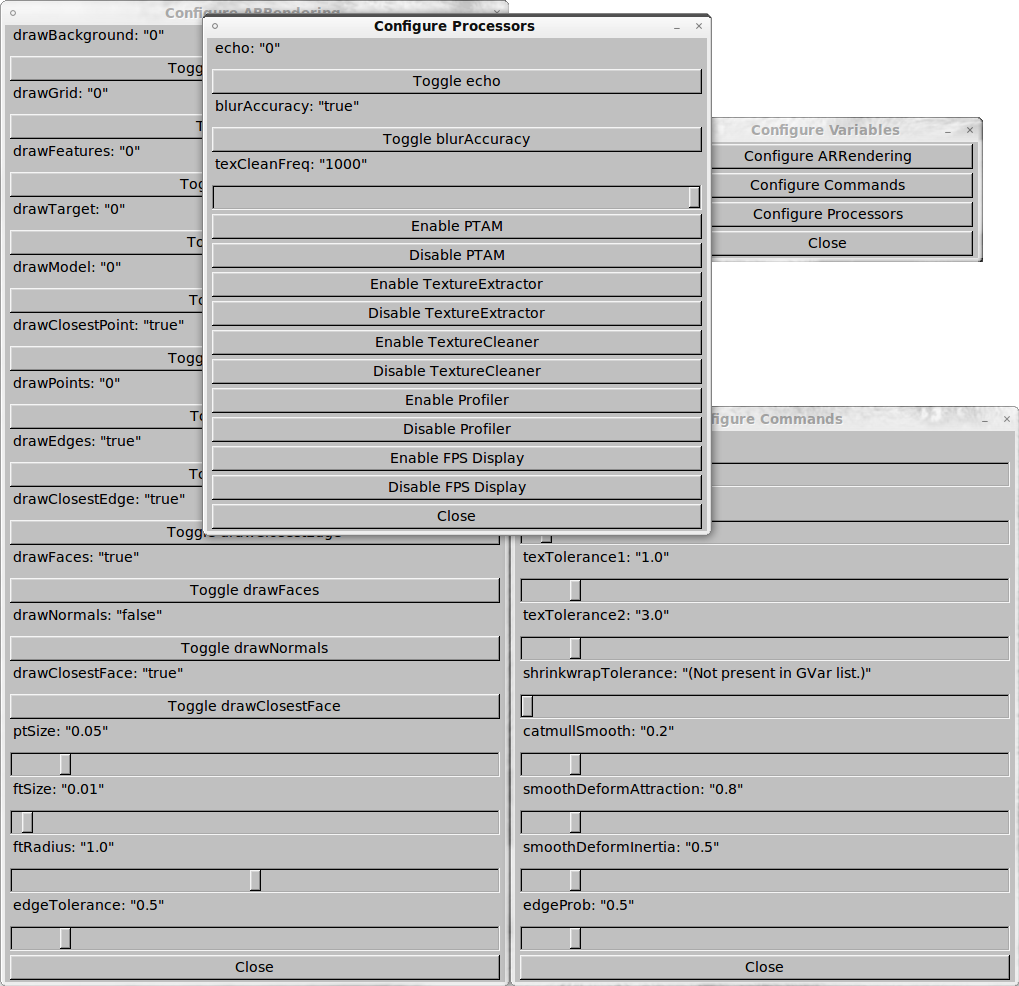
\includegraphics[width=340px]{Config}
  \end{center}
  \caption{Sample pages from the Configuration GUI}
  \label{configui}
\end{figure}

The UI toolkit is built on top of the cross-platform Fast Light ToolKit (FLTK: \url{http://www.fltk.org/}), with bindings already provided by the GVars command interface. This allowed for rapid prototyping of the UI, as well as permitting later adjustments to it; the UI definitions are stored in a separate configuration file (\texttt{configGUI.cfg}) that is reloaded whenever the GUI is invoked with \texttt{config.launch}. Example screens from this are depicted in Figure~\ref{configui}.

The contents of this file can largely be auto-generated by a Bash shell script, parsing default values from the C++ source and constructing a window per file, and a pair of controls (one to monitor the value, and one to adjust it) per window. The tight binding between GVars3 and its FLTK implementation make this file an ideal way to set up this GUI, although it lacks some flexibility in terms of layout and visual design.

\clearpage

\section{Platform Showcase}
\subsection{The Game}
Throughout this project, there has been a conscious focus on the dual design goals of transparent \textit{modularity} and \textit{extensibility}. As architected, the system is capable of being extended in numerous directions, without the user ever having to be aware of the underlying complexity of systems of plugins or the various extension points in the system. In order to demonstrate the extent to which this extensibility can completely alter the behaviour of the system, this Platform Showcase was devised; an opportunity to prove that the system constructed is not only a modelling tool, but also a valid \textit{platform} for building Augmented Reality systems which may rely on models of the environment.

\begin{figure}[t]
    \subfigure[levelHead]{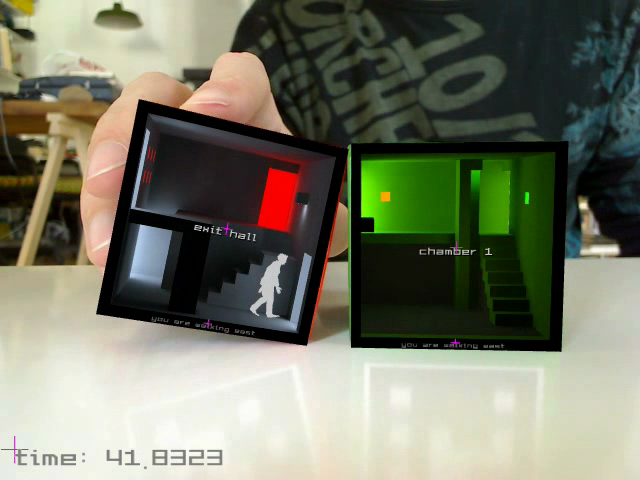
\includegraphics[width=165px]{levelhead3}\label{levelhead}}
    \quad
    \subfigure[SCOPE]{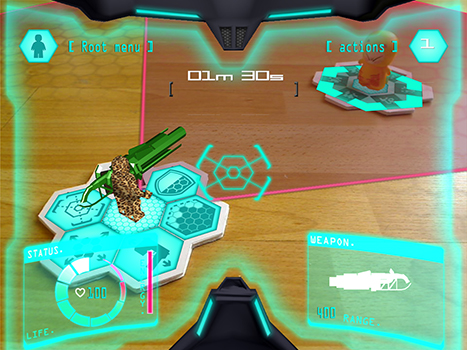
\includegraphics[width=165px]{scope1}\label{scope}}
    \caption{Examples of Augmented Reality Games}
\end{figure}

One increasingly popular application of AR is in entertainment, where it has been used in a variety of videogames. Many of these games, such as the commercial title \textit{Eye of Judgement} \cite{eyeofjudgement} for the PlayStation 3, act like board games with which players interact using specially marked physical cards or tokens. This idea is expanded on in the levelHead \cite{levelhead} project (Figure~\ref{levelhead}), where the board is replaced by a marked cube that the player tilts and spins to control a character. The concept of augmenting simple tokens is studied well in a piece of interaction research by Frantz Lasorne in SCOPE \cite{scope}, pictured in Figure~\ref{scope}.

As mobile phones become more powerful, it is possible for them to perform accurate camera tracking while displaying real-time 3D graphics. This allows more complex game interactions, such as Fanta's Virtual Tennis\cite{fantatennis} advertising game in which players print a marked paper tennis court and play tennis in real-time using two mobile phones as rackets. The Augmented Environments Lab at Georgia Tech has also experimented with several AR games, involving several different methods of interaction.

\begin{wrapfigure}{r}{130pt}
  \vspace{-20pt}
  \begin{center}
    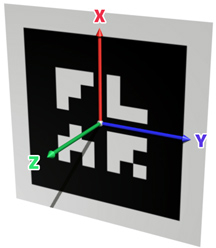
\includegraphics[width=120px]{marker-axis1}
  \end{center}
  \vspace{-10pt}
  \caption{A visual marker used to extract axes}
  \label{markerar}
\end{wrapfigure} 

However, many of these AR experiences are based on techniques popularised by University of Washington ARToolkit \cite{artk}, which was itself based on earlier work \cite{artkpaper} in collaboration between the University of Washington and Hiroshima City University. This so-called \textit{marker based AR} requires tokens (Figure~\ref{markerar}) to extract co-ordinate axes and orient the augmented reality world. These are subject to a number of failure modes, including occlusion or a reduction in image quality due to, for example, motion blur (Figure~\ref{markerfail}). As PTAM tracks the scene based on a much larger number of feature points, if just one collection of points is obscured or untrackable it does not cause the entire track to fail.

\begin{figure}[t]
    \vspace{10pt}
    \subfigure[Marker Occlusion]{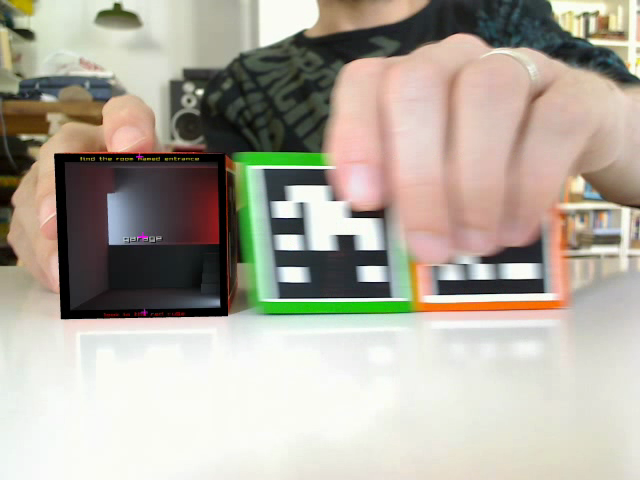
\includegraphics[width=165px]{markerfail_occlusion}}
    \quad
    \subfigure[Poor Image Quality]{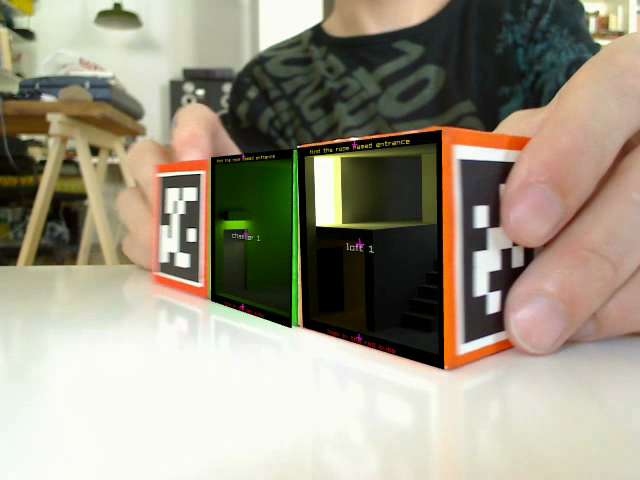
\includegraphics[width=165px]{markerfail_track}}
    \vspace{10pt}
    \caption{Failure modes for marker-based tracking, camera frames extracted from the levelHead demonstration video}
    \vspace{10pt}
    \label{markerfail}
\end{figure}

With this background in mind, the goal is to set up a game engine within the tool's platform, to demonstrate how one can integrate physics, AI, and interactive game elements into a coheisve AR gaming environment.

\subsection{Rendering}
The existing Augmented Reality subsystem was built for extensibility; when the user activates the game mode, the game can safely replace the current instance of the renderer with one which is sensitive to the types of object in the game world. Each \texttt{GameObject} type has a different rendering method; for demonstrative purposes, \texttt{AIUnit}s are rendered as cubes, whilst \texttt{Projectile}s are spherical. As the renderer extends the existing behaviours, the full world model is rendered from the \texttt{Environment} as it is in the normal modelling use case - thus giving the output important results for immersion, such as occlusion or consistency of lighting, ``for free".

\subsection{Real-Time Physics}
In order to offer real-time physics simulation, the Bullet Physics library was selected \cite{bullet}. This collision detection and rigid body physics library was first created by Erwin Coumans, from Sony Computer Entertainment, and has since become the most popular free/open source physics library in use today (rated 3\super{rd} according to \url{http://bulletphysics.org/wordpress/?p=88}, after the expensive closed-source solutions from nVidia and Havok). It has been used in a variety of commercial as well as free games, as well as powering award winning Visual Effects for Hollywood - notably the VES ``Outstanding Supporting Visual Effects in a Feature Motion Picture" for Framestore's work on Sherlock Holmes (\url{http://www.fxguide.com/article597.html} - fBounce is Framestore's custom Maya integration of Bullet). Evalulating the efficiency of this library prior to proceeding with it was vitally important; as PTAM already invokes a fair amount of computation-per-frame, the code for the game engine must be kept as lean as possible. Bullet was found to operate very efficiently, for the complexity of scene likely to be used - certainly well within the bounds of requirements.

\begin{figure}
  \begin{center}
    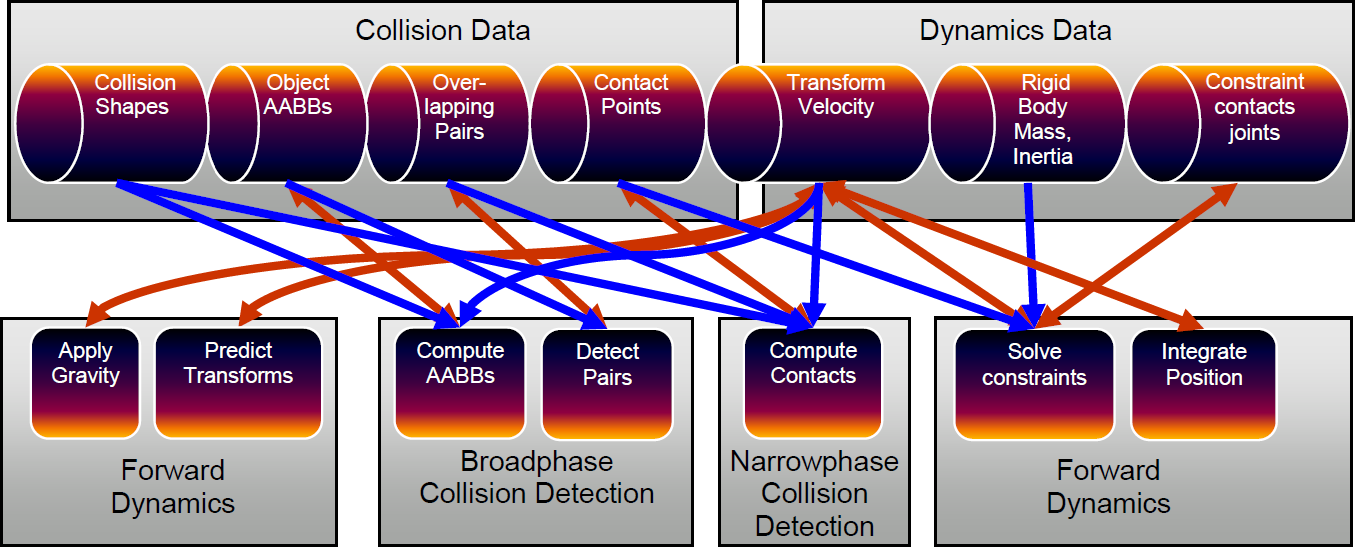
\includegraphics[width=340px]{BulletPipeline}
  \end{center}
  \caption{The Bullet Rigid Body Physics Pipeline (adapted from the Bullet Physics 2.76 SDK Manual)}
  \label{bulletpipe}
\end{figure} 

Bullet's physics pipeline, seen in Figure~\ref{bulletpipe}, starts with the most general simulation elements; it applies gravity to the scene, and predicts where the scene's transforms will move (Forward Dynamics). After this, the configured Broadphase Collision Detection algorithm quickly reduces the set of objects to perform Narrowphase collision detection on; it analyses the Axis Aligned Bounding Box (AABB) of each transform in the scene, and if there is a chance two objects are colliding, they will be passed on for Narrowphase collision. The Broadphase algorithm selected for this demonstration was a Sweep-and-Prune based 3D search - this is much more efficient than a Dynamic AABB Tree, but requires a fixed world size. Finally, the pipeline will solve the precise constraints on the forward dynamics and integrate the final positions of each transform in the scene.

In order to initialise the physics world, it is necessary to transform the model of the world stored in the \texttt{Environment} into a terrain mesh that Bullet can use for collisions. For this purpose, there is a convenient construct in Bullet; the \texttt{btBvhTriangleMeshShape}. This takes as a parameter the \texttt{btTriangleMesh} generated face-by-face from the \texttt{Environment}'s model. Provided vertex ordering is taken into consideration (so that the implicit surface normals for collision are correct), this will provide a suitable rigid body for modelling the scene from a physics standpoint. The shapes of objects mentioned above are carried through to their representation in the physics world, along with modelling their physical properties such as their mass and inertia. Provided the Bullet simulation is allowed to update the pose of the objects, the renderer and game world will always be ``aware" of them in the correct location.

When collisions occur, a custom substep callback that is registered with Bullet causes any suitable game events to be triggered - whether that be ``killing" an object, or racking up points, is a question of creative design. The types of objects can be extracted from the Bullet transforms by retrieving the appropriate \texttt{GameObject} pointer stored within it, using the provided \texttt{btCollisionObject:: getUserPointer()} method.

\subsection{AI Navigation}
In order to make a game environment more compelling, it is desirable that AI units can appear to navigate the world that has been created for them in an intelligent fashion, regardless of the complexity of the terrain facing them. In order to achieve this goal, the A* search algorithm \cite{astar} was selected as an efficient means of path selection, with an option for sensible early termination if either no path can be found, or the computation takes too long. While A* is not guaranteed to find the shortest path, it \textit{is} provably guaranteed to terminate, and be complete. For complex paths, A* may use large amounts of memory - should this prove a problem at a later date, the pathfinding algorithm is encoded in a separate \texttt{AStarSearch} class, and it can be swapped for a much less memory-hungry Iterative Deepening form of A* \cite{idastar}.

In order to perform A* search, the geometry of the model must be simplified from its 3D geometry into a \textit{navigation mesh} - a weighted digraph representing the available edges to traverse in moving from one node to another. In order to generate this, the \texttt{GameFactory} examines the contents of the \texttt{Environment}. From these, it generates \texttt{WayPoint}s - each of which contains the $x$, $y$, $z$ co-ordinates in world-space, as well as lists of the \texttt{Waypoint}s that are traversable, and the distance to them. A \texttt{Waypoint} is added for each \texttt{Point}, and on the centre of each \texttt{PolyFace}. Finally, links are made between \texttt{Waypoint}s based on the gradient along the candidate edge; if it is too steep, then the edge cannot be traversed. In this way, the contours of the terrain are observed when trying to navigate from one position to another. Candidate links are generated from every \texttt{Edge} in the \texttt{Environment}, from the centre of each \texttt{PolyFace} to each of its vertices, and from each point on a face to each other face that is considered planar with it (as discussed previously, using \texttt{Environment::findPlanarFaces}).

Finally, all of these \texttt{Waypoint}s are encoded in a \texttt{WorldMap}, which provides an interface for finding the nearest \texttt{Waypoint} to a given set of 3D co-ordinates. It can also ``tidy up" the \texttt{Waypoint} graph, by removing those points which cannot be reached by any traversal (i.e. a node in the digraph with zero edges).

\subsection{Game Director \& Demo Gameplay}
The final component of the game world is the \texttt{Director}: it controls the flow of the game, and maintains the state of the player's score. In this case, it is a fairly simple affair; over time, it randomly ``spawns" \texttt{AIUnit}s at a random point on one edge of the game world, and tells them to navigate to the far side - ideal for playing on a desk, in a similar fashion to popular Flash-based ``desktop tower defence" games. If an \texttt{AIUnit} reaches the far side, the player loses 300 points. The player can try and stop this by launching projectiles from their handheld camera - if one hits an \texttt{AIUnit} they gain 10 points, and if they knock one off the edge of the game world they earn 100 points. The mechanics are simple, but as a showcase of what a full-time games developer could do with the technology, it provides valuable evidence of the suitability of this sort of technology for recreational gameplay.

\clearpage

\section{Evaluation}
In order to ascertain the extent to which the finished product meets these criteria, carefully defined evaluation must be undertaken. It is not sufficient that the implementation detailed should accomplish the stated goals - there must be a methodology defined to ascertain how \textit{well} it accomplishes those goals. Therefore, two different types of evaluation will be undertaken; end-to-end acceptance testing, and numerical analysis of the accuracy of the result.

\subsection{Acceptance Testing}
The various tools described in Section~\ref{cmdTools} are each an experiment in user interaction. As this is an entirely novel user interface, it is valuable to consider each of the available styles of interacting with the model, with respect to their usability and utility to a modeller.

\begin{itemize}
\item{\textbf{Vertex Manipulation}: It is vital that this most fundamental form of interaction works well; to this end, a fair amount of testing and iterative improvement went into its design throughout the development process. Provided there is a sufficiently prominent feature, it is very quick and almost trivial to place a point in 3D space. The ``coloured balls" targetting system makes it easy to see where the candidate points are, and obvious where the created vertex will be placed. However, there is one critically important caveat; if PTAM does not register a feature where the user desires a vertex, they must choose the "next best" option, which could be a fair distance away. This problem is exacerbated by PTAM's reliance only on the Shi-Tomasi \cite{shitomasi} corner detection algorithm for feature analysis. An extension of PTAM has been described by its original author \cite{ptamedges} which considers not only corners, but also edgelets in its feature map, in an effort to improve its agility. Unfortunately, at the time of writing this version of PTAM is unavailable to the general public, and thus could not be integrated with the rest of the modelling system to test to what extent it would improve the modelling process.

Again, the UI cues as to vertex selection make it clear which vertex will be deleted or moved by the other vertex tools. However, as mentioned previously moving a vertex accurately can be quite challenging. The \textit{``freemove"} variant of the tool permits completely unencumbered motion - but it is hard to tell how much the point has moved in the camera's view axis. For this reason, it is possible to constrain the motion to be only in one axis at a time - an improvement in some cases, but often requires adjustment from each of the tools in turn to achieve the desired translation. This led to the creation of the \textit{third} option (as sure an indicator as any that this interface problem hasn't been solved!): to first identify an axis of motion, and then place the target point anywhere on this axis. This is perhaps the most versatile form of movement, as it permits the user to accurately predict where the point will end up, and by aiming their camera at the same point from two separate views they will almost certainly get the vertex placed where it should be. It is then that slight tweaks from the other tools can be useful to correct the position of the vertex by only a small amount.
}

\item{\textbf{Edge Manipulation}: The closest point of approach basis for edge selection works just as well as the vertex selection, and uses similar visual cues. Such consitency should help to significantly lower the barrier to entry for newcomers learning to use the system. Edge connection is a simple enough primitive operation that nothing can realistically go wrong; it is resilient to user mistakes such as edge loops, and reconnecting already connected edges. No failure cases have been found in which a valid \texttt{PolyFace} is \textit{not} constructed automatically. When the wrong edge is added, it is easy to remove, helping to keep the software resilient; a user should never have to restart an entire model due to a simple mistake.

\begin{figure}
  \begin{center}
    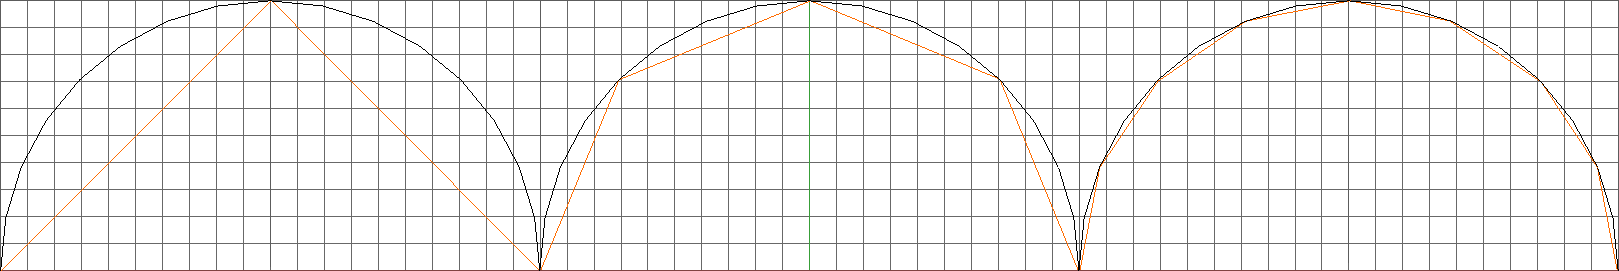
\includegraphics[width=340px]{EdgeRefinement}
  \end{center}
  \caption{A 2D example of refining a curve by manual edge bisection}
  \label{refine}
\end{figure} 

When modelling curves or other complex geometry, the edge bisection tool allows iterative refinement of the curve without too much complexity; see Figure~\ref{refine} for an example of this in practice.}

\item{\textbf{Plane Manipulation}: A variety of features use whole-plane detection to manipulate the model. This detection tends to work well; no cases have been found in which it will incorrectly select non-planar faces. Moving these planes is similar to moving points; keeping the plane a fixed distance from the camera makes it easy to move the plane around. One limitation of the implementation of plane movement is that it won't allow a user to \textit{rotate} the plane - it remains parallel to its original pose. In many cases this is desirable - particularly when extruding the face of an object, as it helps the user be more accurate. In fact, most cases that might benefit from rotating a plane can be more accurately fixed with the vertex movement tools already evaluated, since the inaccuracy would likely be down to just one or two vertices, not a consistent error in all of those on the plane. Therefore, while this is a limitation, the improved accuracy it offers the most probable use cases makes it a limitation worth maintaining.

Extruding a plane is easy to achieve, and because of the rotation invariance of \texttt{plane.move} it is easy to see from multiple angles before placing the final extruded plane's position. The plane split feature provides much the same user experience as edge bisection above. However, it creates more polygons per split than bisecting an edge. Furthermore, through experimentation it has become apparent that few real-world objects can benefit from this mode of editing; most refinement opportunities exist on the edges of a mesh, not in the centre of a face.

The final plane manipulation tool to discuss is that for revolving about an axis. This tool poses an interesting challenge; as already discussed, it is difficult to place vertices on objects with non-corner features. A prime example of this would be a wine bottle; plenty of smooth curves, and very few corners. As a result of this, it is difficult to place vertices on the mesh with sufficient accuracy to make this tool as powerful as it should be. The tool itself works more-or-less exactly as one would wish - but only small errors in placement of the axis can result in a wildly incorrect mesh. 

%TODO: image to illustrate the problem?
}

\item{\textbf{Whole-Mesh Editing}: Moving an entire mesh will be a rare occurence in general usage; perhaps when loading it from disk, or if the object being modelled were to move (although here it would be easier to move the object than the model!). Nevertheless, the feature is available, and it works as expected - with the same rotation invariance as the plane movement.

Scaling a mesh is again likely only to be useful when loading from hard disk. The user interaction for this primitive is very obvious to a user; as they drag the camera from the original pose, it ``feels" just like moving a single point, except the entire mesh is scaled with it. It is valuable to note that this tool will not allow a user to scale a mesh by a different factor in each axis. If it were to do so, it would be far harder to use, and it is not immediately clear with the current tool set when this functionality would be necessary.

Subdivision and smooth deformation are something of a ``mixed bag"; it is important that the user has experience using them, to know when it is suitable to use them. Subdivision can be very useful on a very smooth mesh, essentially performing the same work as \texttt{edge.bisect} but in an automated fashion on the entire model at once. The smooth deformation mode does not work so well; for small deformations there is (we find in real-world testing) little need to ``pull" all of the points simultaneously, and large deformations are quite unlikely. Future work, however, could investigate using a similar approach to do so-called ``voxel sculpting" to start from a primitive shape (cube, cylinder, etc) and work towards a smooth mesh by ``pulling" voxels as if the mesh were modelling clay. This approach is taken by the GPGPU accelerated modelling tool, 3D-Coat (\url{http://www.3d-coat.com/}).
}

\item{\textbf{Texture Application \& Repair}: As the texture application in the system is completely automated, the user should rarely need to concern themselves with how it works. In general, the distortion of textures for display works fairly well; even frames captured at quite oblique angles are mapped quite accurately. However, as discussed earlier and seen in Figure~\ref{camblur}, occasionally captured frames are blurred - in these cases, it is easy for the user to identify these and have the texture replaced. As the ``interaction primitive" for this is the same as interacting with planes, as evaluated above, using this tool should not require any extra practice or training for a user, keeping the entire texture system as low-impact as possible. To this end, experiments were also run with running the \texttt{texture.clean} command at regular intervals, to help repair texture discontinuities (as in Figure~\ref{texclean}), as a \texttt{VisionProcessor}. This worked very well for simple models, but can significantly reduce the framerate when the model becomes too complex. Future work on the efficiency of this method, by introducing further memoisation may well alleviate the problem.
}

\item{\textbf{Saving \& Loading}: There are two formats supported for saving and loading; ``code" and ``obj". The former was originally written as a debugging solution, showing how the GVars3-based command system can be used to quickly serialise a model, and even more easily load it back from disk. However, ``code" has a major limitation; it has no support for saving or loading any texture data on disk. However, the format is verbose and easy to understand and edit, since it takes the same format as the commands in the original system.

Wavefront's OBJ format, on the other hand, is far more versatile, supporting a wide variety of material styles; both flat-colour and texture. However, due to the limited use-case of this modelling software, the export will always create the same type of material; a single textured mesh. Whilst the OBJ format can specify any number of materials to apply to a given set of faces (with each face receiving at most one material), the \texttt{obj.load} command will only support one; the last specified material and material database (MTL file) in the imported OBJ file. This limitation makes it suitable for importing geometry with a single colour or texture - however if the system were to be expanded into a ``commercial grade" product rather than an academic research prototype, this is the sort of limitation on its functionality that should be enhanced. Other such limitations might include support for the full gamut of TARGA images, as well as for non-triangulated meshes (presumably these would be parsed, and then each face converted to triangles before being added to the \texttt{Environment}).
 }
\end{itemize}

\subsection{Accuracy}
\begin{figure}
  \begin{center}
    \subfigure[Modelling example - Desk Surface]{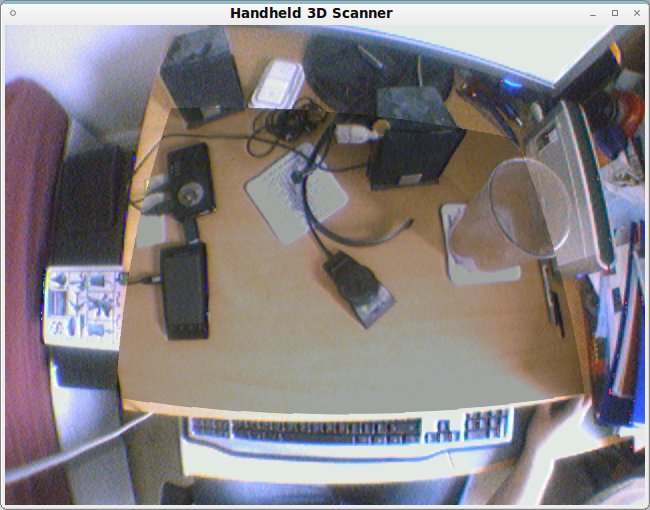
\includegraphics[width=160px]{DeskTest}\label{desktest}}
    \hspace{10px}
    \subfigure[Error Map Pre-Modelling (0.7\%)]{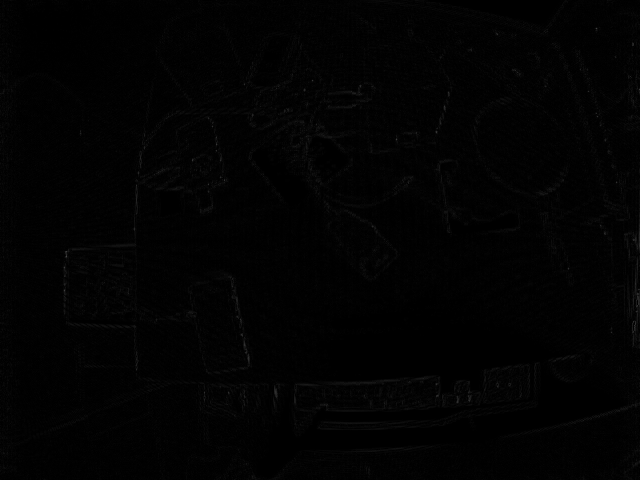
\includegraphics[width=160px]{DeskErrorBlank}\label{errorblank}}
    \subfigure[Error Map With Model (7.2\%)]{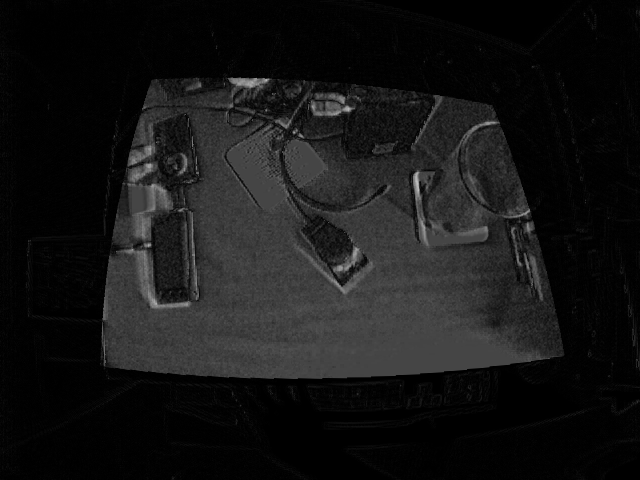
\includegraphics[width=165px]{DeskErrorModel}\label{errormodel}}
    \hspace{10px}
    \subfigure[Error Map Intensity Scale]{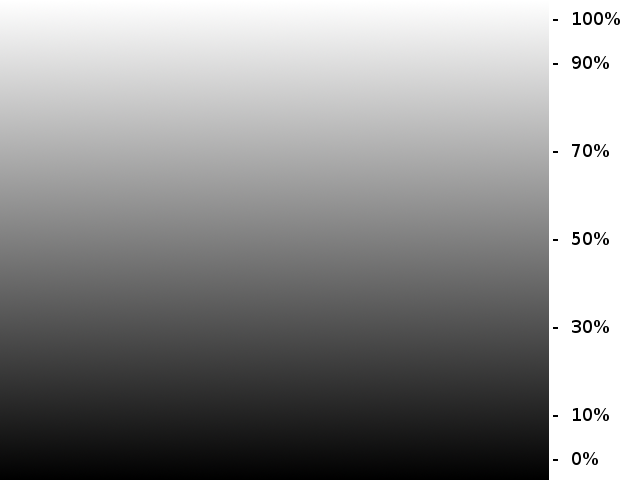
\includegraphics[width=160px]{ErrorMapScale}\label{errorscale1}}
  \end{center}
  \caption{Example error maps}
  \label{errormaps}
\end{figure} 
The numerical analysis of the system's accuracy is altogether less straightforward, as there is no perfect ``gold standard" approach against which the final product can be measured. Furthermore, an artistic ``from scratch" model against which to compare would be both hard to find and not necessarily created with geometric accuracy in mind. If the hardware were available, the geometry that the system outputs can be compared against the point-cloud generate by a LIDAR scanner. This would have the distinct advantage of testing the geometry separately from the texture - however, is infeasible at this time. To some extent, the correctness of texture mapping can be inspected visually; however, a numerical approach to all of the above would be desirable. To this end, an approach which compares the augmented-reality frame and the source camera frame from a few different perspectives would test the accuracy of the complete system; geometry, texture mapping, AR rendering, and even camera calibration. Of course, this means that if any one of these is deficient then the whole system will be deemed inaccurate. 

In order to do this, \texttt{glReadPixels} was used to retrieve the contents of the AR rendered framebuffer into a CVD \texttt{Image\textless Rgb\textless byte\textgreater \textgreater}. By putting this code into a \texttt{VisionProcessor}, it would have access to the original camera frame, in the same format, and could compare the two pixel-by-pixel (bearing in mind the reverse ordering of OpenGL's rows; (0,0) in OpenGL is the bottom left of the frame, while the camera frames put the origin at the top left). By averaging the difference between corresponding pixels, a percentage difference between the images can be discerned. Furthermore, by recording the pixel-by-pixel average differences, a greyscale \textit{error map} can be saved to disk, showing where the errors between frames are strongest. An example of this error map can be seen in Figure~\ref{errormaps}.

\begin{figure}
  \begin{center}
    \subfigure[Error Map Pre-Modelling (0.1\%)]{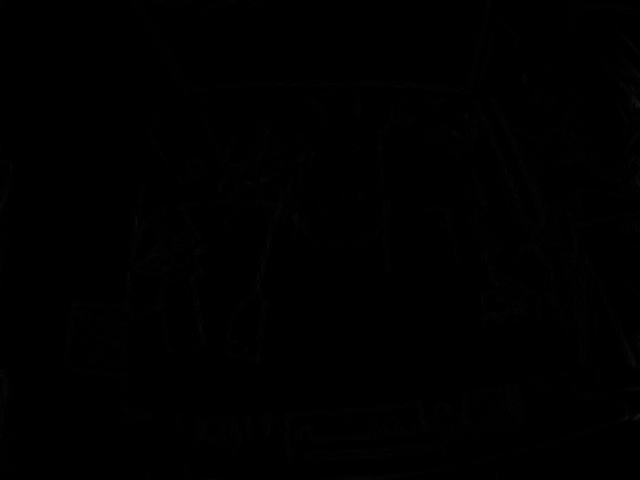
\includegraphics[width=160px]{DeskErrorBlank2}\label{errorblank2}}
    \hspace{10px}
    \subfigure[Error Map With Model \& UI (12.9\%)]{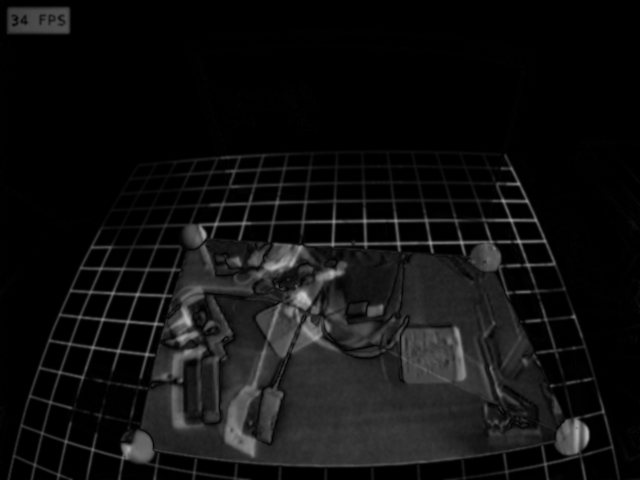
\includegraphics[width=160px]{DeskErrorModelUI}\label{errormodelui}}
    \subfigure[Error Map With Model only (5.5\%)]{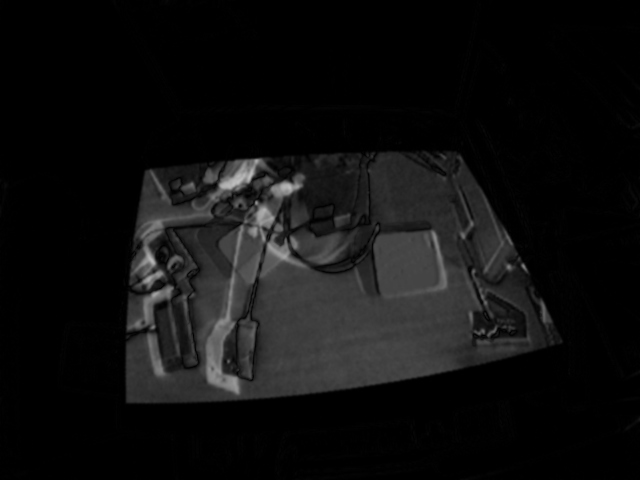
\includegraphics[width=160px]{DeskErrorModel2}\label{errormodel2}}
    \hspace{10px}
    \subfigure[Error Map Intensity Scale]{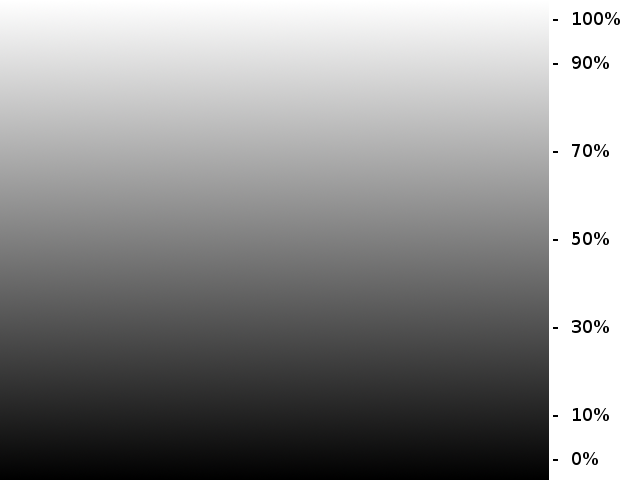
\includegraphics[width=160px]{ErrorMapScale}\label{errorscale2}}
  \end{center}
  \caption{Example error maps, with blurring}
  \label{errormaps2}
\end{figure} 

From analysing these error maps, we can see that the average error across the surface of the desk is around 27\%, with peaks of up to 70\%. However, even when there is no model (as in Figure~\ref{errorblank}), there are clear errors to be seen, mostly on the edges of objects - resulting in a typical ``at rest" error of 7.2\%. This will, most likely, be a result of inaccuracy in either the camera calibration, or the UFB projection matrix used to re-project the camera frames for rendering in OpenGL. However, this minor amount of error could easily be amplified during tracking and texture projection to result in the inaccuracies seen above. One potential solution to this problem is to apply a gaussian convolution matrix to blur both the camera frame and the system's rendered output prior to comparing the two. This should reduce the amount of error due to mis-calibration, leaving a more accurate map of the system's error in its place. Examples of the output from pre-blurring the frames can be seen in Figure~\ref{errormaps2}, using a convolve matrix with $\sigma ~=~ 1.0$. As one might expect, this provides a much better indicator of accuracy - with no UI elements on screen, the error fell to 0.1\%. The average error for this map method on the desk image is closer to 23\% now, a not insignificant improvement.

Of course, this highlights a problem with this approach to accuracy testing - as it is experimental itself, it is difficult to know to what extent \textit{it} can be trusted to deliver a valid judgement of the system's accuracy!

\begin{figure}
  \begin{center}
    \subfigure[Error Histogram Pre-Modelling (0.1\%)]{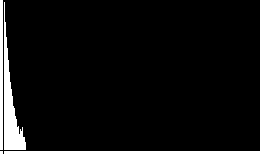
\includegraphics[width=160px]{HistogramBlank}\label{histblank}}
    \hspace{10px}
    \subfigure[Error Histogram With Model \& UI (12.9\%)]{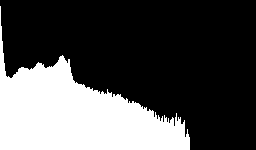
\includegraphics[width=160px]{HistogramModel}\label{histmodel}}
  \end{center}
  \caption{Example error histograms, from the maps in Figure~\ref{errormaps2}}
  \label{histograms}
\end{figure} 

While the percentage error is easy to digest, the error map gives much more detailed information. Ideally, a measure somewhere between the two should provide an easy to compare metric, that provides more detailed information than just a percentage error. In order to do this, Figure~\ref{histograms} shows histograms generated showing the frequency of each amount of error. These make it easy to see that the errors present with a blank model are all present below a peak of 9\%, while those in the modelled case exhibit errors up to 74\% - although under 0.03\% of the image exhibits errors over 70\%. By way of contrast, approximately 40\% of the frame exhibits an error of under 10\%.

%Another approach would be to perform feature detection on the source and AR camera frames, and estimate the motion of co-occurrent features between the two; any features that are not within the model would not have moved, but those which \textit{were} modelled, would be expected to exhibit some form of motion. 

\subsection{Usability}
A third factor that remains unmeasured is the extent to which a new user can pick up the software and learn to use it; one aspect of this is documentation, the other a highly qualitative ``user friendliness". This can hypothetically also be tested, by giving the system to a small cross-section of different users and observing how readily they learn to use it. Worthy of note here is the relative difficulty with which most users learn 3D packages, such as Maya or 3D Studio Max - most 3D tools are highly complex, with many months of learning curve. If a user can pick this system up and start using it to model and texture objects inside of an hour then it should rate quite highly on the usability scale!

\subsection{Performance}
A final key aspect for consideration is the performance of the system. Not only must it remain performant under usual modelling scenarios, but if it is to be used as a platform for other software it is important that its performance characteristics are well understood. The primary form of performance we will consider is the framerate of the software in use, measured in Frames Per Second (FPS). 

\begin{figure}
  \begin{center}
    \subfigure[]{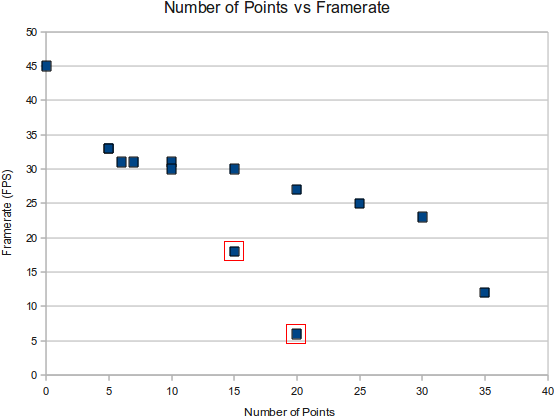
\includegraphics[width=160px]{PointsVsFramerate}\label{pointrate}}
    \hspace{10px}
    \subfigure[]{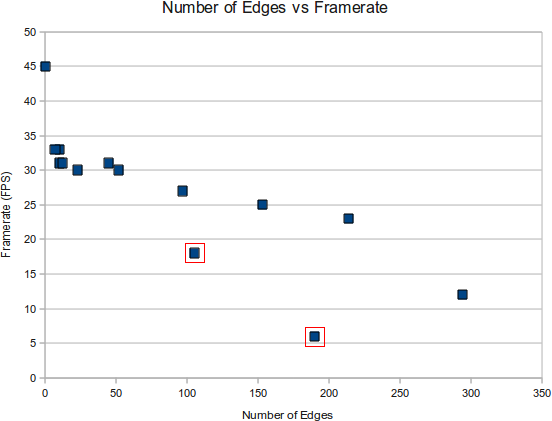
\includegraphics[width=160px]{EdgesVsFramerate}\label{edgerate}}
    \subfigure[]{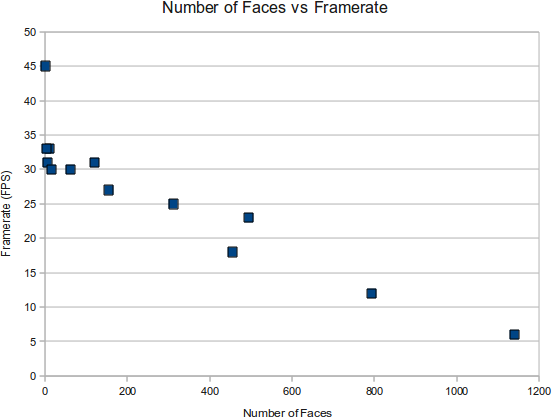
\includegraphics[width=165px]{FacesVsFramerate}\label{facerate}}
  \end{center}
  \caption{Framerate results of the first analysis of mesh complexity}
  \label{framerate}
\end{figure} 

In order to produce models of various resolution to test how well the system scales, an extra command was created. This command would add a number of new \texttt{Point}s to the \texttt{Environment}, and connecting each added \texttt{Point} to every existing point with probability defined by a GVars3 controlled variable, \texttt{edgeProb}. Finally, the resulting size of the three aspects of the model (points, edges, and faces) were recorded after each command invocation. The framerate observed was taken as an approximate average of those calculated while panning the camera around the model - ensuring that PTAM was performing fresh tracking, and the rate shown was ``fair". Whilst the camera was stable, many sizes of model would often exhibit higher framerates than those recorded here; this appeared to be a compound result of PTAM's efficiency, and an OpenGL optimisation of the rendering. The tables of results are given below, with the graphs generated from these data in Figure~\ref{framerate}. The first section of data were generated with an \texttt{edgeProb} of 1, whilst the second were formed from an \texttt{edgeProb} of 0.5.

\begin{center}
\begin{tabular}{| c | c | c || c |} 
\hline
\textbf{Points}	& \textbf{Edges}	& \textbf{Faces}	& \textbf{Framerate} \\
\hline
\hline
0	& 0	& 0	& 45 \\
5	& 10	& 10	& 33 \\
10	& 45	& 120	& 31 \\
15	& 105	& 455	& 18 \\
20	& 190	& 1140	& 6 \\
\hline
\hline
0	& 0		& 0		& 45 \\
5	& 7		& 3		& 33 \\
6	& 10	& 5		& 31 \\
7	& 12	& 5		& 31 \\
10	& 23	& 15	& 30 \\
15	& 52	& 61	& 30 \\
20	& 97	& 155	& 27 \\
25	& 153	& 311	& 25 \\
30	& 214	& 495	& 23 \\
35	& 294	& 794	& 12 \\
\hline
\end{tabular}
\end{center} 

In analysing these graphs, we can clearly see that as the overall complexity of the model increases, the framerate decreases in proportion. However, the first two graphs (Figures~\ref{pointrate} and \ref{edgerate}) also have clear dips in framerate (highlighted) corresponding to the more complex models in the \textit{first} data set. The fact that these spurious discontinuities are not present in Figure~\ref{facerate} suggest that the primary cause of the drop in framerate is the increase in number of faces. This hypothesis is borne out by the profiling data, which show a significant proportion of each frame's rendering devoted to rendering the textured \texttt{PolyFace}s.

\begin{figure}
  \begin{center}
    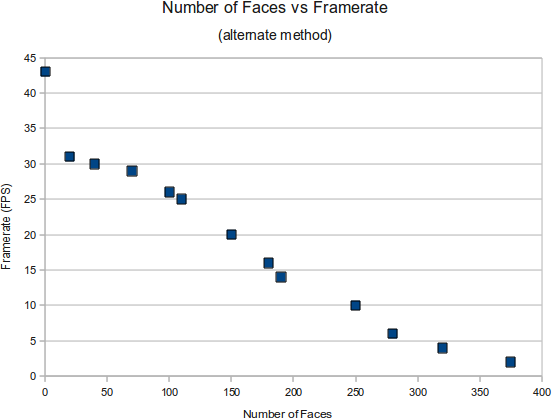
\includegraphics[width=340px]{FacesVsFramerate2}
  \end{center}
  \caption{Second analysis of effect of face count on framerate}
  \label{facesrate2}
\end{figure}

With this in mind, a second random mesh generator was written. Instead of focussing on number of points, it can be tasked to generate a mesh of a given number of faces, by iteratively generating a new \texttt{PolyFace} from the current new point, as well as the previous two generated points. The mesh is not as heavily connected as in the previous generator, but arguably grows at a more realistic rate of faces in relation to number of points and edges. The raw data for this analysis is again below, with the graph generated from it shown in Figure~\ref{facesrate2}.

\begin{center}
\begin{tabular}{| c || c |} 
\hline
\textbf{Number of Points}	& \textbf{Framerate} \\
\hline
\hline
0	& 43 \\
20	& 31 \\
40	& 30 \\
70	& 29 \\
100	& 26 \\
110	& 25 \\
150	& 20 \\
180	& 16 \\
190	& 14 \\
250	& 10 \\
280	& 6 \\
320	& 4 \\
375	& 2 \\
\hline
\end{tabular}
\end{center}

\clearpage

\section{Conclusion}
As was highlighted at the very beginning of this project, there are a plethora of reasons for a user to want to generate a 3D model, from user-generated content in games, through to complex high-precision CAD. There is no way that any tool can claim to please all of the people, all of time, but it seems clear from the evaluation above that there is a definite niche for the system described in this document. Its performance has been found to be highly satisfactory, with rare drops in frame-rate, attributable to infeasibly complex models. Should it be made into a more commercial product, further development on the rendering subsystem to utilise more advanced OpenGL constructs should alleviate almost all of these difficulties. The true success has been in prototyping a variety of natural user interactions with the system. Informal user studies have shown that the average user can start modelling within just a few minutes of having the system demonstrated to them, with more advanced use cases becoming comfortable for them after a brief period of practice.

The experiments in this novel UI have largely been a success; some more experimental tools have been omitted from this document, since they have not in some cases come to fruition - but most of the interaction primitives discussed are useful in at least a subset of cases. Furthermore, it has become clear that the system is, in fact, capable of \textit{more} than it was originally designed for. The motivation for it was originally to construct a manual modelling tool that was not subject to the foibles of automated vision-based scanning systems. In so doing, it has become quite possible to model entirely novel objects with this interactive, hand-held tool - not just those in the scene in front of the user. Since the system has to be able to cope with adjustments to scenes in areas where there are no discernable features to track, it is capable of modelling parts of, or even entire, objects that are not actually present in the scene before the camera - the only limits are the proficiency and imagination of the user.

Overall, while this research has provided some interesting results and analysis of a new style of user interaction, it has not proved suitable for creating high-resolution, high-accuracy models. Nevertheless; when it is clear (as it seems to be here) that a novel approach can \textit{help} rather than \textit{hinder} an artist's creativity, it becomes easy to argue that it is an approach worthy of refinement, and even further study.

\clearpage

\section{Further Work}
As we have argued, the work described herein could well provide an interesting foundation for further research and development. Some of the most promising work today utilises many more techniques from computer vision; from recent developments in fully automated dense reconstruction \cite{denserecon}, through to more interaction-based approaches, such as in the Jiim interface to VideoTrace \cite{jiim}. These both strive for fully interactive performance, though with very differenct approaches to user interaction. It would be interesting to investigate a hybrid approach; perhaps using simple constraints defined through the interaction model described here as a more semantically aware base mesh for a dense reconstruction.

Another type of improvement that should significantly enhance the system is also vision-based; awareness of a greater number of features in the scene. This could be just for the interaction (for example, using the edglet-enhanced version of PTAM discussed in the Evaluation), or to do a more VideoTrace-style automatic enhancement and fitting of edges to features in the scene (especially edgelets).

The Jiim interface mentioned above uses PTAM to create an augmented reality ``viewer" for objects, but maintains the mouse-based tracing interface described in the previous VideoTrace work. This is also a potentially interesting avenue to pursue - as a mock-up of this, Appendix~\ref{melar} describes a MEL (\textit{Maya Embedded Language}) script that can be added to a button on Autodesk's Maya software for loading a mesh from Maya into this tool for viewing or adjusting in an AR view. This would allow any Maya user to model creatively in their existing tool, and then explore their model in AR; this could be an even more compelling experience if support were added for 3D VR goggles, perhaps attaching the camera to these so that the visualisation becomes completely natural.

The final area that could have significant value in further development is exploring usability enhancements. As a research prototype, there's no doubt that there are features a user may like access to, for example;
\begin{itemize}
\item{Undo \& Redo stack}
\item{File Open / Save dialogs (for browsing)}
\item{Friendlier configuration GUI}
\item{Option to switch between a fully-automated mode}
\item{Automatic object translation / rotation detection and mesh realignment (making it easier to model all sides of an object)}
\end{itemize}

In short, there are a huge variety of directions this work could be taken in, almost all of which would be sure to expand on its utility and enhance its usability. That the approach taken here may serve as a foundation for such future work (both in spirit and even architecturally, from an engineering standpoint) is a rewarding conclusion to draw indeed.


\clearpage
\renewcommand*{\refname}{\section{References}}
\bibliography{Report}
\bibliographystyle{dcu}

\clearpage
\appendix
\section{User-Configurable Parameters}
\label{configparams}
\begin{verbatim}
//
// Modelling Settings
//

// ARDriver:
drawBackground = true 
drawGrid = true 

// ARPointRenderer:
drawPoints = true 
drawFeatures = true 
drawModel = true 
drawTarget = true 
ptSize = 0.05 
drawClosestPoint = true 
ftSize = 0.01 
ftRadius = 1.0
drawEdges = true 
drawClosestEdge = true 
drawFaces = true 
drawNormals = false 
drawClosestFace = true 
drawClosestPlane = true 

// Commands:
ftRadius = 1.0 
edgeTolerance = 0.5 
edgeTolerance = 0.5 
planeTolerance = 0.1 
revolveFaces = 10 
planeTolerance = 0.1
texTolerance1 = 1.0 
texTolerance2 = 3.0 
catmullSmooth = 0.2 
smoothDeformAttraction = 0.8 
smoothDeformInertia = 0.5 
edgeProb = 0.5 

// Processors:
echo =  false 
texCleanFreq = 1000 
blurAccuracy = true 
\end{verbatim}

\clearpage

\begin{verbatim}
//
// Game Settings
//

// AIUnit:
aiMass = 5 
aiPatience = 100000 
aiSpeed = 20 

// Director:
game.impactScore = 0 
game.deathScore = 100 
game.goalScore = -300 
spawnTolerance = 0.3 
spawnFreq = 3000 
spawnProb = 0.0001 

// GameFactory:
maxGradient = 1.0 
physicsScale = 1000 

// GameRenderer:
drawModel = true 
drawWaypoints = true 
drawProjectiles = true 
drawUnits = true 
waypointSize = 0.02 

// Hooks:
physicsStep = 1.f/60.f 
gravity = -15 
pushScale = 80 

// Projectile:
projectileMass =  0.4 
\end{verbatim}

\clearpage

\section{MEL Script to Invoke Tool for Viewing}
\label{melar}
\noindent
\ttfamily
\hlstd{}\hllin{\ 1\ }\hlcom{/{*}{*}}\\
\hllin{\ 2\ }\hlcom{\ {*}\ Launch\ the\ tool\ with\ a\ triangulated\ form\ of\ the}\\
\hllin{\ 3\ }\hlcom{\ {*}\ current\ model(s)\ loaded}\\
\hllin{\ 4\ }\hlcom{\ {*}/}\hlstd{}\\
\hllin{\ 5\ }\hlkwa{global\ proc\ }\hlstd{launchViewer}\hlopt{()\ \usebox{\hlboxopenbrace}}\\
\hllin{\ 6\ }\hlstd{}\hlstd{\ \ \ \ }\hlstd{}\hlkwc{\$file\ }\hlstd{}\hlopt{=\ }\hlstd{}\hlstr{"/tmp/curr.obj"}\hlstd{}\hlopt{;}\\
\hllin{\ 7\ }\hlstd{}\hlstd{\ \ \ \ }\hlstd{\\
\hllin{\ 8\ }}\hlstd{\ \ \ \ }\hlstd{}\hlkwa{string\ }\hlstd{}\hlkwc{\$toDelete}\hlstd{}\hlopt{{[}{]};}\\
\hllin{\ 9\ }\hlstd{}\hlstd{\ \ \ \ }\hlstd{}\hlkwa{for}\hlstd{}\hlopt{(\ }\hlstd{}\hlkwc{\$obj\ }\hlstd{}\hlkwa{in\ }\hlstd{}\hlstr{`ls\ {-}l\ {-}type\ "mesh"`}\hlstd{\ }\hlopt{)\ \usebox{\hlboxopenbrace}}\\
\hllin{10\ }\hlstd{}\hlstd{\ \ \ \ \ \ \ \ }\hlstd{}\hlkwa{string\ }\hlstd{}\hlkwc{\$tri}\hlstd{}\hlopt{{[}{]}\ =\ }\hlstd{}\hlstr{`polyTriangulate\ {-}ch\ 1\ \$obj`}\hlstd{}\hlopt{;}\\
\hllin{11\ }\hlstd{}\hlstd{\ \ \ \ \ \ \ \ }\hlstd{}\hlkwc{\$toDelete}\hlstd{}\hlopt{{[}}\hlstd{size}\hlopt{(\ }\hlstd{}\hlkwc{\$toDelete\ }\hlstd{}\hlopt{){]}\ =\ }\hlstd{}\hlkwc{\$tri}\hlstd{}\hlopt{{[}}\hlstd{}\hlnum{0}\hlstd{}\hlopt{{]};}\\
\hllin{12\ }\hlstd{}\hlstd{\ \ \ \ }\hlstd{}\hlopt{\usebox{\hlboxclosebrace}}\\
\hllin{13\ }\hlstd{}\hlstd{\ \ \ \ }\hlstd{\\
\hllin{14\ }}\hlstd{\ \ \ \ }\hlstd{}\hlslc{//\ Export\ the\ triangulated\ mesh\ to\ OBJ\ format}\\
\hllin{15\ }\hlstd{}\hlstd{\ \ \ \ }\hlstd{}\hlkwb{file}\hlstd{\ \ }\hlkwb{}\hlstd{}\hlopt{{-}}\hlstd{typ\ }\hlstr{"OBJexport"}\hlstd{\ }\hlopt{{-}}\hlstd{ea\ }\hlkwc{\$file}\hlstd{}\hlopt{;}\\
\hllin{16\ }\hlstd{}\hlstd{\ \ \ \ }\hlstd{\\
\hllin{17\ }}\hlstd{\ \ \ \ }\hlstd{}\hlslc{//\ Undo\ the\ triangulation\ by\ removing\ polyTriangulate}\\
\hllin{18\ }\hlstd{}\hlstd{\ \ \ \ }\hlstd{}\hlslc{//}\hlstd{\ \ \ }\hlslc{nodes\ from\ scene}\\
\hllin{19\ }\hlstd{}\hlstd{\ \ \ \ }\hlstd{}\hlkwa{for}\hlstd{}\hlopt{(\ }\hlstd{}\hlkwc{\$del\ }\hlstd{}\hlkwa{in\ }\hlstd{}\hlkwc{\$toDelete\ }\hlstd{}\hlopt{)\ \usebox{\hlboxopenbrace}}\\
\hllin{20\ }\hlstd{}\hlstd{\ \ \ \ \ \ \ \ }\hlstd{}\hlkwa{if\ }\hlstd{}\hlopt{(\ }\hlstd{}\hlkwb{objExists}\hlstd{}\hlopt{(\ }\hlstd{}\hlkwc{\$del\ }\hlstd{}\hlopt{)\ )}\\
\hllin{21\ }\hlstd{}\hlstd{\ \ \ \ \ \ \ \ \ \ \ \ }\hlstd{}\hlkwb{delete\ }\hlstd{}\hlkwc{\$del}\hlstd{}\hlopt{;}\\
\hllin{22\ }\hlstd{}\hlstd{\ \ \ \ }\hlstd{}\hlopt{\usebox{\hlboxclosebrace}}\\
\hllin{23\ }\hlstd{}\hlstd{\ \ \ \ }\hlstd{\\
\hllin{24\ }}\hlstd{\ \ \ \ }\hlstd{}\hlslc{//\ Invoke\ tool\ \&\ instruct\ to\ load\ file}\\
\hllin{25\ }\hlstd{}\hlstd{\ \ \ \ }\hlstd{}\hlkwc{\$pipe\ }\hlstd{}\hlopt{=\ }\hlstd{popen}\hlopt{(\ }\hlstd{}\hlstr{"/path/to/Modeller"}\hlstd{}\hlopt{,\ }\hlstd{}\hlstr{"w"}\hlstd{\ }\hlopt{);}\\
\hllin{26\ }\hlstd{}\hlstd{\ \ \ \ }\hlstd{}\hlkwa{if\ }\hlstd{}\hlopt{(\ }\hlstd{}\hlkwc{\$pipe\ }\hlstd{}\hlopt{!=\ }\hlstd{}\hlnum{0\ }\hlstd{}\hlopt{)\ \usebox{\hlboxopenbrace}}\\
\hllin{27\ }\hlstd{}\hlstd{\ \ \ \ \ \ \ \ }\hlstd{fprint}\hlopt{(\ }\hlstd{}\hlkwc{\$pipe}\hlstd{}\hlopt{,\ }\hlstd{}\hlstr{"obj.load\ "}\hlstd{}\hlopt{+}\hlstd{}\hlkwc{\$file\ }\hlstd{}\hlopt{);}\\
\hllin{28\ }\hlstd{}\hlstd{\ \ \ \ \ \ \ \ }\hlstd{fclose}\hlopt{(\ }\hlstd{}\hlkwc{\$pipe\ }\hlstd{}\hlopt{);}\\
\hllin{29\ }\hlstd{}\hlstd{\ \ \ \ }\hlstd{}\hlopt{\usebox{\hlboxclosebrace}}\\
\hllin{30\ }\hlstd{}\hlopt{\usebox{\hlboxclosebrace}}\\
\hllin{31\ }\hlstd{}\\
\hllin{32\ }\hlcom{/{*}{*}}\\
\hllin{33\ }\hlcom{\ {*}\ Assume\ the\ tool\ saved\ a\ model\ to\ the\ default}\\
\hllin{34\ }\hlcom{\ {*}\ location,\ delete\ the\ current\ model\ and\ load}\\
\hllin{35\ }\hlcom{\ {*}\ a\ tweaked\ model\ from\ disk}\\
\hllin{36\ }\hlcom{\ {*}/}\hlstd{}\\
\hllin{37\ }\hlkwa{global\ proc\ }\hlstd{loadFromViewer}\hlopt{()\ \usebox{\hlboxopenbrace}}\\
\hllin{38\ }\hlstd{}\hlstd{\ \ \ \ }\hlstd{}\hlkwc{\$file\ }\hlstd{}\hlopt{=\ }\hlstd{}\hlstr{"/path/to/Modeller/scanner\textunderscore model.obj"}\hlstd{}\hlopt{;}\\
\hllin{39\ }\hlstd{}\hlstd{\ \ \ \ }\hlstd{\\
\hllin{40\ }}\hlstd{\ \ \ \ }\hlstd{}\hlslc{//\ Delete\ the\ current\ mesh}\\
\hllin{41\ }\hlstd{}\hlstd{\ \ \ \ }\hlstd{}\hlkwa{for}\hlstd{}\hlopt{(\ }\hlstd{}\hlkwc{\$del\ }\hlstd{}\hlkwa{in\ }\hlstd{}\hlstr{`ls\ {-}l\ {-}type\ "mesh"`}\hlstd{\ }\hlopt{)\ \usebox{\hlboxopenbrace}}\\
\hllin{42\ }\hlstd{}\hlstd{\ \ \ \ \ \ \ \ }\hlstd{}\hlkwa{if\ }\hlstd{}\hlopt{(\ }\hlstd{}\hlkwb{objExists}\hlstd{}\hlopt{(\ }\hlstd{}\hlkwc{\$del\ }\hlstd{}\hlopt{)\ )}\\
\hllin{43\ }\hlstd{}\hlstd{\ \ \ \ \ \ \ \ \ \ \ \ }\hlstd{}\hlkwb{delete\ }\hlstd{}\hlkwc{\$del}\hlstd{}\hlopt{;}\\
\hllin{44\ }\hlstd{}\hlstd{\ \ \ \ }\hlstd{}\hlopt{\usebox{\hlboxclosebrace}}\hlstd{\ \ }\hlopt{}\\
\hllin{45\ }\hlstd{}\hlstd{\ \ \ \ }\hlstd{\\
\hllin{46\ }}\hlstd{\ \ \ \ }\hlstd{}\hlslc{//\ Load\ the\ saved\ OBJ\ file}\\
\hllin{47\ }\hlstd{}\hlstd{\ \ \ \ }\hlstd{}\hlkwb{file\ }\hlstd{}\hlopt{{-}}\hlstd{import\ }\hlopt{{-}}\hlstd{type\ }\hlstr{"OBJ"}\hlstd{\ }\hlkwc{\$file}\hlstd{}\hlopt{;}\\
\hllin{48\ }\hlstd{}\hlopt{\usebox{\hlboxclosebrace}}\hlstd{}\\
\mbox{}
\normalfont
\normalsize
\end{document}          
